\documentclass{elsarticle}

\usepackage{lineno,hyperref}
%\usepackage{refcheck}
\modulolinenumbers[5]
% % % % % % % % % % % % % % % % % % % % % % % % % % %
%added by Mostafa
% Package 'amsmath' pre-loaded by Vahid
\RequirePackage{amsmath}

%\documentclass[twocolumn]{svjour3}          % twocolumn
%
%
%Two packages added by Vahid
%\usepackage{cite}
%\usepackage{lineno}
%\linenumbers
%\usepackage{amsmath}
%\usepackage{flexisym}
%\usepackage{algorithmic}
\usepackage{amssymb, bm, mathrsfs, xcolor, hyperref}
\usepackage{graphicx,subfig}
\usepackage[section,subsection,subsubsection]{extraplaceins}
\usepackage[]{algorithm2e}
\usepackage{algpseudocode}% http://ctan.org/pkg/{algorithms,algorithmicx}
\usepackage{placeins}
%\usepackage{stmaryrd}
% Package below added by Vahid to prevent a warning
\usepackage{textcomp}
%\usepackage{gensymb}
%\usepackage[mathscr]{euscript}
%\usepackage{dsfont}
%\usepackage{mathptmx}      % use Times fonts if available on your TeX system
 \usepackage[mathscr]{euscript}
%\usepackage{changes}
\usepackage{epstopdf}
\graphicspath{{Figures/}, {Figures/Mandel/}}
%\usepackage{todonotes}
%\renewcommand{\todo}{}
%\newtheorem{theorem}{Theorem}[section]
%\newtheorem{remark}{remark}[theorem]

% insert here the call for the packages your document requires
%\usepackage{latexsym}
% etc.
%
% please place your own definitions here and don't use \def but
% \newcommand{}{}


%\graphicspath{{CO2_Paper_Draft/figures}}
\usepackage{booktabs} % Allows the use of \toprule, \midrule and \bottomrule in tables
%\usepackage{float}
%\usepackage{subcaption}
%\usepackage{subfig}
%\usepackage{color}
\setlength{\textfloatsep}{10pt plus 1.0pt minus 2.0pt}
\setlength{\intextsep}{10pt plus 1.0pt minus 2.0pt}
\setlength{\floatsep}{10pt plus 1.0pt minus 2.0pt}
\setlength{\dbltextfloatsep}{10pt plus 1.0pt minus 2.0pt}
\setlength{\dblfloatsep}{10pt plus 1.0pt minus 2.0pt}

% Added by Vahid
\usepackage{listings}
\usepackage{color}
\usepackage{changes}
\usepackage{lipsum}% <- For dummy text
\definechangesauthor[name={Vahid}, color=orange]{Vahid}
\setremarkmarkup{(#2)}

\definecolor{dkgreen}{rgb}{0,0.6,0}
\definecolor{gray}{rgb}{0.5,0.5,0.5}
\definecolor{mauve}{rgb}{0.58,0,0.82}

\lstset{frame=tb,
  language=Python,
  aboveskip=3mm,
  belowskip=3mm,
  showstringspaces=false,
  columns=flexible,
  basicstyle={\small\ttfamily},
  % numbers=none,
  %Added by Vahid
  numbers=left,
  stepnumber=1,
  numberstyle=\tiny\color{gray},
  keywordstyle=\color{blue},
  commentstyle=\color{dkgreen},
  stringstyle=\color{mauve},
  breaklines=true,
  breakatwhitespace=true,
  tabsize=3
}

\DeclareMathOperator{\divergence}{div}
\DeclareMathOperator{\sign}{sign}
\DeclareMathOperator{\dist}{dist}
\DeclareMathOperator{\supp}{supp}
\DeclareMathOperator{\trace}{tr}
\DeclareMathOperator{\vol}{vol}
\DeclareMathOperator{\dev}{dev}
\DeclareMathOperator{\argmin}{arg min}

% The line below added by Vahid to prevent a warning
%\hypersetup{final}
%\include{definitions}
%\newtheorem{remark}{remark}[theorem]


\usepackage[utf8]{inputenc}
\usepackage[english]{babel}
\usepackage{amsthm}
\newtheorem{remark}{Remark}

% % % % % % % % % % % % % % % % % % % % % % % % % %
%\usepackage{changes}
\usepackage{todonotes}
\newcommand{\comment}[1]{{\color{blue}\vspace{5 mm}\par \noindent
		\marginpar{\textsc{Comment}} \framebox{\begin{minipage}[c]{0.95
					\textwidth} \tt #1 \end{minipage}}\vspace{5 mm}\par}}

\journal{Journal of Natural Gas Science and Engineering}

%%%%%%%%%%%%%%%%%%%%%%%
%% Elsevier bibliography styles
%%%%%%%%%%%%%%%%%%%%%%%
%% To change the style, put a % in front of the second line of the current style and
%% remove the % from the second line of the style you would like to use.
%%%%%%%%%%%%%%%%%%%%%%%

%% Numbered
%\bibliographystyle{model1-num-names}

%% Numbered without titles
%\bibliographystyle{model1a-num-names}

%% Harvard
%\bibliographystyle{model2-names.bst}\biboptions{authoryear}

%% Vancouver numbered
%\usepackage{numcompress}\bibliographystyle{model3-num-names}

%% Vancouver name/year
%\usepackage{numcompress}\bibliographystyle{model4-names}\biboptions{authoryear}

%% APA style
%\bibliographystyle{model5-names}\biboptions{authoryear}

%% AMA style
%\usepackage{numcompress}\bibliographystyle{model6-num-names}

%% `Elsevier LaTeX' style
\bibliographystyle{elsarticle-num}
%%%%%%%%%%%%%%%%%%%%%%%

\begin{document}

\begin{frontmatter}

\title{Numerical of Thermo-hydro- mechanical modeling of CO$_2$ fracturing by the phase field approach}
%\tnotetext[mytitlenote]{Fully documented templates are available in the elsarticle package on \href{http://www.ctan.org/tex-archive/macros/latex/contrib/elsarticle}{CTAN}.}

%% Group authors per affiliation:
%\author{Mostafa Mollaali\fnref{myfootnote}}
%\address{Radarweg 29, Amsterdam}
%\fntext[myfootnote]{Since 1880.}

%% or include affiliations in footnotes:
\author[mymainaddress]{Vahid Ziaei-Rad}
\author[mysecondaryaddress]{Mostafa Mollaali}
%\ead[url]{www.elsevier.com}


%\ead[url]{www.elsevier.com}

\author[mysecondaryaddress]{Yongxing Shen\corref{mycorrespondingauthor}}
\cortext[mycorrespondingauthor]{Corresponding author}
\ead{yongxing.shen@sjtu.edu.cn}

\address[mymainaddress]{Department of Civil Engineering, Isfahan University of Technology, Isfahan 84156-83111, Iran}
\address[mysecondaryaddress]{University of Michigan -- Shanghai Jiao Tong University Joint Institute, Shanghai Jiao Tong University,	Shanghai, China}

\begin{abstract}

\end{abstract}

\begin{keyword}
%\texttt{elsarticle.cls}\sep \LaTeX\sep Elsevier \sep template
CO$_2$ fracturing \sep  CO$_2$ fluid flow \sep  phase field
\MSC[2010] 65K10
\end{keyword}

\end{frontmatter}

\linenumbers

%\todo[inline]{YS to VZR: Whenever ready, please update your email address to the one with your current affiliation.}

%\todo[inline]{YS: We have to fix the multiply defined labels. Check the log.\\
%Vahid: I have fixed some warnings. Others mostly come from Section \ref{sec:num-examples} which we will do soon later then.}

\section{Introduction}

The objective of the paper at hand is to propose a phase field model to investigate the effect of thermo-hydro-mechanical CO$_2$ fracturing in saturated porous media.


%\section{Mathematical model}\label{sec:Math_model}

\subsection{Porous medium deformation and fracture propagation}\label{Sec:Phase_Field}
In this section, 
we briefly recapitulate the basic notations and the underlying equations of the phase field method for pressurized fractures in brittle materials.

\subsubsection{Variational formulation of brittle fracture}
Let $\Omega\subset\mathbb{R}^\eta$, $\eta=2,3$ be an open Lipchitz domain occupied by a porous medium with a lower-dimensional fracture $\mathcal{C}\in\mathbb{R}^{\eta-1}$, see Figure \ref{Fig:comput_domain}. Let the displacement field be $\bm{u}:\Omega\rightarrow\mathbb{R}^\eta$. Let $\Gamma_D,\Gamma_N\subseteq \partial\Omega$ be such that $\Gamma_D\cup\Gamma_N=\partial\Omega$ and $\Gamma_D\cap\Gamma_N=\emptyset$. Further, let $\bm{u}_D: \Gamma_D\rightarrow\mathbb{R}^2$ and $\bm{t}_N: \Gamma_N\rightarrow\mathbb{R}^2$ be prescribed displacement and traction boundary conditions, respectively. We denote by $\Gamma_B$ the boundary of a borehole, and by $Q_g:\Gamma_B\rightarrow\mathbb{R}$ the fluid source. We have $\Gamma_P=\partial\Omega\setminus\Gamma_B$, and let $p_D:\Gamma_p\rightarrow\mathbb{R}$ be prescribed pressure. Also, $\mathbf{b}:\Omega\rightarrow\mathbb{R}^\eta$ is the body force per unit volume exerted to the solid.
\begin{figure}[htbp]
	\centering
	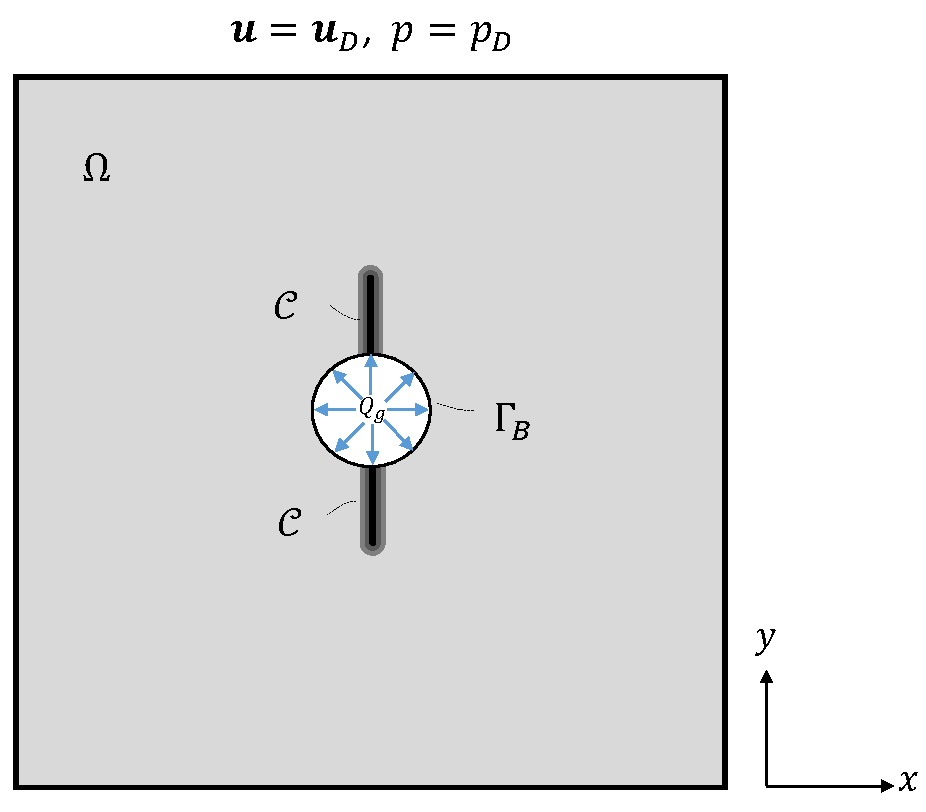
\includegraphics[width=0.8\textwidth]{omega_insitu2}
	\caption{A bounded reservoir domain $\Omega$ with a lower-dimensional crack $\mathcal{C}\in\mathbb{R}^{\eta-1}$ (left) and its diffuse approximation.}
	\label{Fig:comput_domain}
\end{figure}
\comment{We also need to define prescribed boundary condition for $T$.}
The linearized strain tensor takes the form:
\begin{equation}\label{Eq:epsilon}
	\begin{aligned}
		\bm{\varepsilon}(\bm{u})=\frac12(\nabla\bm{u}+\nabla\bm{u}^T)
	\end{aligned}
\end{equation}
which can be decomposed into two parts:
\begin{equation}\label{Eq:epsilon_decomp}
\begin{aligned}
	\bm{\varepsilon}(\bm{u}) = \bm{\varepsilon_e}+\bm{\varepsilon_{\theta}}.
\end{aligned}
\end{equation}
Here, $\bm{\varepsilon_e}$ and $\bm{\varepsilon_{\theta}}$ are the elastic and thermal strain tensors, respectively. We assume that $\bm{\varepsilon_{\theta}}$ is proportional to the temperature $\theta$ via:
\begin{equation}\label{Eq:epsilon_theta}
	\begin{aligned}
		\bm{\varepsilon_{\theta}} = \beta(\theta-\theta_0)\mathbf{I},
	\end{aligned}
	\end{equation}
where $\theta_0$ is a reference temperature, $\beta$ is the linear expansion coefficient of the material, and $\mathbf{I}$ is the \deleted{second-order} identity tensor.

The energy of a poroelastic medium $\Omega$ with a crack $\mathcal{C}$ reads:
\begin{equation}\label{Eq:E}
\begin{aligned}
E(\bm{u},\mathcal{C}):= \frac12 \int_{\Omega\setminus\mathcal{C}} \mathbb{C}\left(\bm{\varepsilon}_e(\bm{u})-\frac{\alpha}{3K}p\mathbf{I}\right):\left(\bm{\varepsilon}_e(\bm{u})-\frac{\alpha}{3K}p\mathbf{I}\right)\; d\Omega - W(\bm{u}),
\end{aligned}
\end{equation}
where $\mathbb{C}\in\mathbb{R}^4$ denotes the fourth-order Gassman tensor, and $\alpha\in[0,1]$ and $p$ are the Biot's coefficient and the pore pressure, respectively. Also, $K=E/[3(1-2\nu)]$ where $E$, $\nu$ are Young's modulus and Poisson's ratio, respectively.
The external work $W(\bm{u})$ is defined as:
\begin{equation}\label{Eq:External}
	\begin{aligned}
		W(\bm{u}):=\int_{\Omega} \bm{b} \cdot \bm{u} \; d\Omega+\int_{\Gamma_N} \bm{t}_N\cdot \bm{u} \; d\Gamma - \int_{\mathcal{C}} p\bm{n}\cdot[\bm{u}] \; d\Gamma,
	\end{aligned}
\end{equation}
where $\bm{n}\cdot[\bm{u}]\geq 0$ represents the displacement discontinuity on the fracture surface so that the term $\int_{\mathcal{C}} p\bm{n}\cdot[\bm{u}] \; d\Gamma$
%third term on the right hand side of \eqref{Eq:External}
is the work done by the absorbed gas on the fracture surface.

The variational approach to fracture first proposed by Francfort and Marigo \cite{bourdin2008variational} defines the total energy as the sum of the potential energy and the surface energy required to create a fracture set $\mathcal{C}$. Let $\mathcal{H}^{\eta-1}(\mathcal{C})$ denote the lower-dimensional Hausdorff measure of $\mathcal{C}$. Taking the constant $G_c\in\mathbb{R}^+$ as the strain energy released per unit length of fracture extension, the total energy will be formed as:
\begin{equation}\label{Eq:Pi}
	\begin{aligned}
		\Pi[\bm{u},\mathcal{C}]=E(\bm{u},\mathcal{C})+G_c\mathcal{H}^{\eta-1}(\mathcal{C}).
	\end{aligned}
\end{equation}
In the variational setting, the Griffith criteria will be the
minimum of the total energy \eqref{Eq:Pi} with respect to any admissible displacement field $\bm{u}$ and any fracture set $\mathcal{C}$ subject to an irreversibility condition, i.e., the crack can never heal.

\subsubsection{Regularized variational formulation of brittle fracture}
To develop a numerical method to approximate \eqref{Eq:Pi}, we need to replace the sharp description of crack $\mathcal{C}$ with a phase field representative, where the phase field is denoted as $d:\Omega\rightarrow[0,1]$. Following the approach presented by Ambrosio and Tortorelli \cite{ambrosio1990approximation, ambrosio1992approximation}, one can approximate $\mathcal{H}^{\eta-1}(\mathcal{C})$ with the help of an elliptic functional as:
\begin{equation}\label{Eq:Gamma_ell}
\begin{aligned}
\mathcal{C}_\ell[d]:=\frac{1}{4c_{\omega}}\int_\Omega\left(\frac{\omega(d)}{\ell} + \ell \nabla d\cdot\nabla d\right) d\Omega,  
\end{aligned}
\end{equation}
%where $d:\Omega\rightarrow[0,1]$ is the phase field parameter. 
In particular, regions with $d = 0$ and $d = 1$ correspond to the intact and fully broken materials, respectively.
We denote by $\ell>0$ the regularization length scale, which may also be interpreted as a material property, e.g., the size of the process zone.
In \eqref{Eq:Gamma_ell}, we consider $c_\omega=\int_{0}^{1} \sqrt{\omega(d)}$ as a normalization constant such that as $\ell\rightarrow 0$, $\mathcal{C}_\ell[d]$ converges to the length of sharp crack $\mathcal{H}^{\eta-1}(\mathcal{C})$. Also, we choose $\omega(d)=d^2$, see \cite{tanne2018crack, Bourdin2014014301} for more elaborations.

The solid endures partial loss of stiffness due to the presence of fractures. To model this effect, the poroelastic energy needs to be degraded with respect to the evolution of the phase field. Also note that as the damaged material responds differently to tension and compression, we should let only a part of the poroelastic energy be degraded. Following \cite{amor2009regularized}, we assume that both volumetric expansion and deviatoric deformation contribute to crack propagation but not volumetric compression. 
A decomposition of $\bm{\varepsilon}_e$ into volumetric and deviatoric components reads:
\begin{equation}
	\begin{aligned}
		\vol\bm{\varepsilon}_e := \frac{1}{\eta} (\trace\bm{\varepsilon}_e) \mathbf{I}_{\eta}, \quad
		\dev\bm{\varepsilon}_e := \bm{\varepsilon}_e - \vol\bm{\varepsilon}_e,
	\end{aligned}
\end{equation}
where $\vol\bm{\varepsilon}_e$ will also be decomposed into expansion and compression parts such that
\begin{equation}
	\begin{aligned}
		\vol\bm{\varepsilon}_e=\vol_+\bm{\varepsilon}_e+\vol_-\bm{\varepsilon}_e, \quad \vol_{\pm}\bm{\varepsilon}_e=\frac{1}{\eta}\langle \trace \bm{\varepsilon}_e \rangle_{\pm},
	\end{aligned}
\end{equation}
where $\langle a\rangle_\pm:=\left(|a|\pm a\right)/2$ for all $a\in\mathbb{R}$.
%On this basis, we can rewrite \eqref{Eq:E} as:
On this basis, we rewrite \eqref{Eq:E} with decomposition of the poroelastic energy into expansion/compression volumetric and deviatoric parts as:
\begin{equation*}\label{Eq:E_Amor}
	\begin{aligned}
		E(\bm{u},\mathcal{C})&:= \frac12 \int_{\Omega\setminus\mathcal{C}} \mathbb{C}\Big\langle\vol\bm{\varepsilon}_e-\frac{\alpha}{3K}p\mathbf{I}\Big\rangle_{+}:\Big\langle\vol\bm{\varepsilon}_e-\frac{\alpha}{3K}p\mathbf{I}\Big\rangle_{+}\; d\Omega \\&+
		\frac12 \int_{\Omega\setminus\mathcal{C}} \mathbb{C}\Big\langle\vol\bm{\varepsilon}_e-\frac{\alpha}{3K}p\mathbf{I}\Big\rangle_{-}:\Big\langle\vol\bm{\varepsilon}_e-\frac{\alpha}{3K}p\mathbf{I}\Big\rangle_{-}\; d\Omega \\&+ \int_{\Omega\setminus\mathcal{C}} \mathbb{C}\dev\bm{\varepsilon}_e:\dev\bm{\varepsilon}_e\; d\Omega - W(\bm{u}),
	\end{aligned}
\end{equation*}
To take into account any pre-existing crack, we define $\Gamma_d\subset\overline{\Omega}$ to be a set with Hausdorff dimension $\eta-1$, and $d_0:\Gamma_d\rightarrow[0,1]$ as the Dirichlet boundary condition for $d$. Thus, we define the affine space of the admissible $\bm{u}$ and $d$ fields:
\begin{equation}\label{Eq:Dissipative_admissible}
\begin{aligned}
\mathscr{S}_u &:= \left\{\bm{u}\in H^1\left(\Omega; \mathbb{R}^\eta\right) \middle|
\bm{u} = \bm{u}_D \text{ on } \Gamma_D
\right\}, \\
\mathscr{S}_d &:= \left\{d\in H^1(\Omega) \middle|
0 \le d \le 1 \text{ a.e.}, d = d_0 \text{ on } \Gamma_d
\right\}. \\
%\mathscr{S}_d &:= H^1(\Omega).
\end{aligned}
\end{equation}
On this basis, the regularized variational formulation for brittle fracture of the solid reads: Find $\left(\bm{u}\times d \right)\in\mathscr{S}_{\bm{u}}\times\mathscr{S}_d$ that minimizes the following total energy:
\begin{equation}\label{Eq:Dissipative_functional}
\begin{aligned}
\Pi(\bm{u},d)&:= \frac12 \int_{\Omega} \mathbb{C}\Big\langle\sqrt{g(d)}\vol\bm{\varepsilon}_e-\frac{\alpha}{3K}p\mathbf{I}\Big\rangle_{+}:\Big\langle\sqrt{g(d)}\vol\bm{\varepsilon}_e-\frac{\alpha}{3K}p\mathbf{I}\Big\rangle_{+}\; d\Omega \\&+
\frac12\int_{\Omega}\mathbb{C}\Big\langle\vol\bm{\varepsilon}_e-\frac{\alpha}{3K}p\mathbf{I}\Big\rangle_{-}:\Big\langle\vol\bm{\varepsilon}_e-\frac{\alpha}{3K}p\mathbf{I}\Big\rangle_{-}\; d\Omega \\&+
\int_{\Omega} g(d)\mathbb{C}\dev\bm{\varepsilon}_e:\dev\bm{\varepsilon}_e\; d\Omega\\&+
\frac{G_c}{4c_{\omega}}\int_\Omega \left(\frac{\omega(d)}{\ell} + \ell \nabla d\cdot\nabla d\right)\;d\Omega- W(\bm{u}),
\end{aligned}
\end{equation}
where $g(d)$ is a degradation function that satisfies $g(0)=1$, $g(1)=0$, and $g'(d)<0$. A usual choice is $g(d)=(1-d)^2$ \cite{Bourdin2000797}. Note that the requirement $g'(d)<0$ comes from the underlying irreversibility condition (the fracture can never heal) in time:
\begin{equation}\label{Eq:irreversibility}
\partial_t d\geq 0.
\end{equation}
Consequently, modeling of fracture evolution problems leads to {inequality constraints, and sometimes gives rise to a variational inequality formulation}.
Also, note that in this regularized form, the external work in \eqref{Eq:External} is rewritten as:
\begin{equation*}
\begin{aligned}
W(\bm{u}):=\int_{\Omega} \bm{b} \cdot \bm{u} \; d\Omega+\int_{\Gamma_N} \bm{t}_N\cdot \bm{u} \; d\Gamma - \int_{\Omega} p\bm{u}\cdot\nabla d \; d\Omega,
\end{aligned}
\end{equation*}
where $\int_{\Omega} \bm{u}\cdot\nabla d \; d\Omega$ represents the fracture volume \cite{BourdinCFRAC13}.

It can be shown that when $\ell\rightarrow 0$, the regularized formulation $\Gamma-$converges to that with explicit crack representation, i.e., when $\ell\rightarrow0$, the solution to the minimization problem \eqref{Eq:Dissipative_functional} $\Gamma$-converges to that of $d\Pi[\bm{u},\mathcal{C}]=0$, and also $\mathcal{C}_\ell[d]$ converges to $\mathcal{H}^{\eta-1}(\mathcal{C})$. See Bourdin \emph{et al.} \cite{bourdin2008variational} for the proof of the static anti-plane case.

%\paragraph{The choice of $\ell$}
%{Based on an analytical solution for the critical tensile strength $\sigma_\text{cr}$ that a one-dimensional bar can sustain \cite{Bourdin2014014301}, we use the following equation for the choice of $\ell$:}
%\begin{equation}\label{Eq:choice_ell}
%    \begin{aligned}
%        \ell=\frac{3EG_c}{8\sigma_\text{cr}^2},
%    \end{aligned}
%\end{equation}
%where $E$ and $g_c$ can be obtained from regular experiments, while $\sigma_\text{cr}$ can be approximated by the tensile strength $\sigma_t$. Assuming all {other} parameters are known, the formula \eqref{Eq:choice_ell} is able to estimate $\ell$, though the accuracy is unknown for more complex cases.

\subsection{Carbon dioxide as a compressible fluid} \label{Sec:CO2}
Assume the porous medium is saturated by a single-phase gas. We denote by $\phi$ the porosity of the porous medium (the fraction of volume occupied by the gas), and by $\rho_g, \rho_s$ the gas and solid density, respectively. Note that in this paper, the subscripts $s$  and $g$ refer to solid and gas phases, respectively. The mass balance for the gas reads:
\begin{equation}\label{Eq:Mass_fluid}
    \begin{aligned}
        \partial_t\left(\phi\rho_g\right)  +\nabla\cdot\left(\phi\rho_g \mathbf{v}_g\right)&=0  \quad  &\text{in~} \Omega,
    \end{aligned}
\end{equation}
and for the solid phase:
\begin{equation}\label{Eq:Mass_solid}
\begin{aligned}
\partial_t\left(\left(1- \phi\right) \rho_s\right) + \nabla\cdot\left(\left(1- \phi\right)\rho_s \mathbf{v}_s\right)&=0  \quad  &\text{in~} \Omega.
\end{aligned}
\end{equation}
In \eqref{Eq:Mass_fluid} and \eqref{Eq:Mass_solid}, $\mathbf{v}_g$ and $\mathbf{v}_s$ are respectively the absolute value of gas and solid velocity in the bulk.
Multiplying \eqref{Eq:Mass_fluid} by $\frac{1}{\rho_g}$ and \eqref{Eq:Mass_solid} by $\frac{1}{\rho_s}$, we sum up \eqref{Eq:Mass_fluid} and \eqref{Eq:Mass_solid} to obtain:
\begin{equation*}\label{Eq:Mass_sum}
	\begin{aligned}
	&\frac{\phi}{\rho_g}\partial_t\rho_g+\frac{1}{\rho_g}\nabla\cdot\left(\phi\rho_g \mathbf{v}_g\right)+\frac{1-\phi}{\rho_s}\partial_t\rho_s\\
	&+\frac{1}{\rho_s}\left[(1-\phi)\rho_s \nabla \cdot \mathbf{v}_s+\mathbf{v}_s \cdot \nabla \left((1-\phi)\rho_s)\right)\right]=0.
	\end{aligned}
\end{equation*}
By neglecting $\nabla\left(\left(1-\phi\right)\rho_s\right)$, it reads:%(see \cite{lewis1998finite}, section 2.6.3.2),
\begin{equation}\label{Eq:Mass_sum_intmediate}
	\begin{aligned}
        \frac{\phi}{\rho_g }\partial_t\rho_g+\frac{1}{\rho_g}\nabla\cdot\left(\phi\rho_g \mathbf{v}_g\right)+\frac{1-\phi}{\rho_s}\partial_t\rho_s+(1-\phi)\nabla\cdot \mathbf{v}_s=0.
	\end{aligned}
\end{equation}
We introduce an intermediate term $\nabla\cdot\left(\phi\rho_g\mathbf{v}_s\right)$ as follows:
\begin{equation*}
	\begin{aligned}
    	\frac{1}{\rho_g}\nabla\cdot\left(\phi\rho_g \mathbf{v}_s\right)=\frac{1}{\rho_g}\left[\phi\rho_g\nabla\cdot\mathbf{v}_s+\mathbf{v}_s \cdot \nabla\left(\phi\rho_g\right)\right] \approx \phi\nabla\cdot\mathbf{v}_s,
    \end{aligned}
\end{equation*}
Having this, we define $\nabla\cdot\left(\phi\rho_g\mathbf{v}_g\right)$ as:
\begin{equation} \label{Eq:div_vrho_f}
	\begin{aligned}
	    \frac{1}{\rho_g}\nabla\cdot\left(\phi\rho_g\mathbf{v}_g\right)
    	&=\frac{1}{\rho_g}\nabla\cdot\left(\phi\rho_g \mathbf{v}_g\right)-\frac{1}{\rho_g}\nabla\cdot\left(\phi\rho_g \mathbf{v}_s\right)+\phi\nabla\cdot\mathbf{v}_s\\
	    &=\frac{1}{\rho_g}\nabla\cdot\left[\phi\rho_g\left(\mathbf{v}_g-\mathbf{v}_s\right)\right]+\phi\nabla\cdot\mathbf{v}_s.
    \end{aligned}
\end{equation}
By substituting \eqref{Eq:div_vrho_f} in \eqref{Eq:Mass_sum_intmediate}, we obtain:
\begin{equation}\label{Eq:Mass_Conserv_sum_darcy}
\begin{aligned}
\frac{\phi}{\rho_g}\partial_t\rho_g +\frac{1-\phi}{\rho_s}\partial_t\rho_s+\nabla\cdot\mathbf{v}_s+\frac{1}{\rho_g} \nabla\cdot \left[\phi \rho_g \left(\mathbf{v}_g-\mathbf{v}_s \right)\right] =0,  \quad  &\text{in~} \Omega.
\end{aligned}
\end{equation}
%We will rewrite each term of \eqref{Eq:Mass_Conserv_sum_darcy} in terms of $\bm{u}, p, T$.
The first term on the left hand side of \eqref{Eq:Mass_Conserv_sum_darcy} can be written as:
\begin{equation}\label{Eq:diff_rho_f}
\begin{aligned}
\frac{\phi}{\rho_g}\partial_t\rho_g = \frac{\phi}{\rho_g} \left[ \frac{\partial \rho_g}{\partial p}\partial_t p+\frac{\partial \rho_g}{\partial T}\partial_tT\right] = \phi \left[ \beta_p \partial_t p+ \beta_T \partial_tT\right],
\end{aligned}
\end{equation}
where $\beta_p=\rho_g{\partial\rho_g}/{\partial p}$, and $\beta_T=\rho_g{\partial\rho_g}/{\partial T}$.
%\comment{Here, I should see if there is a name for $\beta_p$, $\beta_T$.}
Under non-isothermal conditions, the gas density varies significantly with both pressure and temperature. We {capture} this by an equation of state (EOS) \cite{mahmoud2014development}:
\begin{equation} \label{Eq:EOS}
\rho_g\left( p,T\right)  =\frac{Mp}{Z\left( p,T\right) RT},
\end{equation}
where $M$ denotes the gas molecular weight, and $R$ is the general gas constant. Also, $Z$ is obtained from the following:
\begin{equation*} \label{Eq:Z_EOS}
Z=\left(0.702e^{-2.5T_{pr}} \right) p_{pr}^2 -\left(5.52e^{-2.5T_{pr}} \right) p_{pr}+\left(0.044 T_{pr}^2 -0.164T_{pr} +1.15\right).
\end{equation*}
Here, $p_{pr}=p/p_c$ and $T_{pr}=T/T_c$ are the reduced pressure and temperature, respectively. Note also $p_c$ and $T_c$ denote the critical pressure and temperature.
On this basis, we rewrite $\beta_p$ and $\beta_T$ as follows:
\begin{equation} \label{Eq:partial_density_p_T}
\begin{aligned}
\beta_p=\frac{1}{\rho_g}\frac{\partial \rho_g}{\partial p} &= \frac{1}{p}- \frac{1}{Z} \frac{\partial Z}{\partial p}, \\
\beta_T= \frac{1}{\rho_g}\frac{\partial \rho_g}{\partial T} &= -\frac{1}{T}- \frac{1}{Z} \frac{\partial Z}{\partial T}.
\end{aligned}
\end{equation}
The second term on the left hand side of \eqref{Eq:Mass_Conserv_sum_darcy} reads \cite{lewis1998finite}: %see \cite{lewis1998finite}, Equation 2.190)
\begin{equation}\label{Eq:diff_rho_s}
\begin{aligned}
\frac{1-\phi}{\rho_s} \partial_t\rho_s= \left(\alpha-\phi \right) \frac{1}{K_s} \partial_t p -\beta_s\left(\alpha-\phi \right) \partial_t T - \left(1-\alpha \right)  \nabla \cdot \mathbf{v}_s,
\end{aligned}
\end{equation}
%\comment{Is $K_s$ the same as $k$ in \eqref{Eq:E}?}
where {$K_s$ denotes the bulk modulus of the grain material}, $\beta_s=\frac{1}{\rho_s}\frac{\partial\rho_s}{\partial T}$ is the thermal expansion coefficient for the solid, and $T$ is the absolute temperature.
The third term on the left hand side of \eqref{Eq:Mass_Conserv_sum_darcy} (also the last term of \eqref{Eq:diff_rho_s}) can be written as follows \cite{merxhani2016introduction}:
\begin{equation} \label{Eq:solid velocity}
\begin{aligned}
\nabla \cdot \mathbf{v}_s=\nabla \cdot \dot{\bm{u}}= \dot{\left( \nabla \cdot \bm{u}\right)}=\partial_t\left(\vol\bm{\varepsilon}\right).
\end{aligned}
\end{equation}
The forth term on the left hand side of \eqref{Eq:Mass_Conserv_sum_darcy} can be written in the form of Darcy's law. This law indicates a linear relationship between the relative velocity of gas to solid and the head pressure gradient:
\begin{equation}\label{Eq:Darcy_law}
\begin{aligned}
\mathbf{q} = \phi \left(\mathbf{v}_g-\mathbf{v}_s \right) = -\frac{\kappa}{\mu} \nabla p,
\end{aligned}
\end{equation}
where $\kappa$ is the permeability of rock, and $\mu$ is the dynamic fluid viscosity. 
Note that we neglect the effect of gravity in Darcy's law. %($\rho_f g \nabla z$)

By substituting \eqref{Eq:diff_rho_f}, \eqref{Eq:diff_rho_s}, \eqref{Eq:solid velocity}, and \eqref{Eq:Darcy_law} in \eqref{Eq:Mass_Conserv_sum_darcy}, the governing equation for CO$_2$ flow is written as follows:
\begin{equation}\label{Eq:General_pressure}
\begin{aligned}
\left[\phi\beta_p +\frac{\alpha-\phi}{K_s}\right]\partial_t p+\left[\phi\beta_T-\beta_s(\alpha-\phi)\right]\partial_t T\\+\alpha \partial_t(\vol\varepsilon)+\frac{1}{\rho_g}\nabla\cdot \left(\rho_g\mathbf{q}\right)=0 \quad &\text{in~} \Omega,\\
\rho_g\bm{q} \cdot \mathbf{n} =-Q_g \quad  &\text{on~} \Gamma_B,\\
p = p_D \quad &\text{on~}\Gamma_P.
\end{aligned}
\end{equation}
%where $\Gamma_P=\partial\Omega\setminus\Gamma_B$.
\subsubsection{Calculation of $k$}
\paragraph{Change of $k$ by phase field} As the cracks initiates, the permeability of the solid matrix increases inside the crack. To incorporate this effect into our model, 
we correlate the permeability to phase field by:
\begin{equation} \label{Eq:k_0}
\kappa(d)=\kappa_0+d\left(\kappa_c-\kappa_0 \right),
\end{equation}
where $\kappa_0$, $\kappa_c$ are the permeability of the intact material and the crack, respectively. Hence, a change of permeability is assumed between the intact porous medium ($d=0$) and the crack ($d=1$). In \eqref{Eq:k_0}, $\kappa_c={w_c^2}/{12}$ where $w_c$ is the fracture width.
Let $h_e$ be the mesh size, $\varepsilon_{ii}$ be the components of strain tensor $\bm{\varepsilon}$, and $\bm{n}_c=\frac{\nabla d}{|\nabla d|}=n_{ci}\bm{e}_i$ be the normal vector to crack path. Following \cite{heider2018modeling}, $w_c$ in a 2D setting can be estimated at each quadrature point as:
\begin{equation*}
w_c=\sqrt{\left[h_e\left(1+\varepsilon_{11}\right)n_{c1}\right]^2+\left[h_e\left(1+\varepsilon_{22}\right)n_{c2}\right]^2}.
\end{equation*}
\comment{We can introduce alternative approaches to calculate $w_c$, but it needs to be for each quadrature point.}

\paragraph{Change of $\kappa_0$ by pressure and temperature} The Darcy's law in a viscous flow regime is valid for conventional reservoirs. However, when the average mean free path of the gas molecules is comparable to the pore size containing it, there is a break in continuum theory. This is evaluated by Knudsen number which is defined as the ratio of mean free path of molecules $\lambda$ to a representative path $L$, e.g., mean hydraulic radius of capillaries:
\begin{equation}
\begin{aligned}
\kappa_n=\frac{\lambda}{L}, \quad \lambda=\frac{\mu}{p}\sqrt{\frac{\pi R T}{2M}}, \quad L=2\sqrt{2\tau_h}\sqrt{\frac{\kappa_{\infty}}{\phi}},
\end{aligned}
\end{equation}
where $\tau_h$ is the tortuosity of the shale matrix.
From the Knudsen number we can divide the flow as: continuous flow, slip flow, transition flow, and free molecular flow or Knudsen diffusion.
Sheng \emph{et al.} \cite{Sheng2012} proposed a formulation which incorporates all flow regimes in one single equation to evaluate the permeability $\kappa_0$. It reads:
%The shale permeability is also pressure dependent due to its nano-scale pore structures. Hence, the Darcy's law in its simple form is valid only for the flow in conventional reservoirs, although there are more complicated flow regimes for the shale reservoir, namely slip flow, transition flow, and Knudsen diffusion.
%\comment{More description on flow regimes is needed.}
%Following \cite{Civan2010, Sheng2012}, in this paper we use a formulation which incorporates all flow regimes in one single equation for the calculation of $k$:
\begin{equation}
\begin{aligned}
\kappa_0=\kappa_{\infty}f(\kappa_n),
\end{aligned}
\end{equation}
where $\kappa_{\infty}$ denotes intrinsic permeability. It can be measured using the pressure pulse decay \cite{Sheng2012}. Also, $f(\kappa_n)$ is written as:
\begin{equation}
\begin{aligned}
f(\kappa_n)=\left(1+a\kappa_n\right)\left(1+\frac{4\kappa_n}{1-b\kappa_n}\right),
\end{aligned}
\end{equation}
in which $a, b$ are dimensionless rarefaction and the slip coefficients, respectively. We find $a$ via:
\begin{equation*}
\begin{aligned}
\frac{a}{a_0}-1=\frac{A}{{\kappa_n}^B},
\end{aligned}
\end{equation*}
where $A, B$ are fitting constants. In this paper, we take $a_0=1.358, A=0.1780, B=0.4348$ \cite{Civan2010}.
%where $\lambda$ is given by:
%\begin{equation}
%\begin{aligned}
%\lambda=\frac{\mu}{p}\sqrt{\frac{\pi R T}{2M}}.
%\end{aligned}
%\end{equation}
%Also we take $L$ as below:
%\begin{equation}
%\begin{aligned}
%L=2\sqrt{2\tau_h}\sqrt{\frac{k_{0}}{\phi}},
%\end{aligned}
%\end{equation}
%This formulation works also for non isothermal cases.

\subsection{Energy balance equation} %\cite{Nield2017,lewis1998finite, khoei2012thermo}%%
%\todo[inline]{Mostafa: For more details see: (i) Chapter 2 of \cite{Nield2017} Equations (2.1-2.6), (ii) Chapter 1, section 2.6.3.3 \cite{lewis1998finite}, and  (iii) \cite{khoei2012thermo}}
%In order to derive the thermo-hydro-mechanical formulation, the heat transfer formulation is incorporated into the governing equations of porous saturated media using the energy conserving equation (enthalpy balance) for each phase. The governing equation of heat conduction is derived for a continuous medium from the principle of conservation of heat energy over an arbitrary fixed volume. Based on this principle, the heat increase rate of the system is equal to the summation of heat conduction and heat generation rate in a fixed volume. Applying the Fourier law of heat conduction, the energy balance equation can be written as
We assume that the solid and gas phases are in a state of thermodynamic equilibrium, i.e., the temperature of both phases are equal at each point in the dual-phase system:
\begin{equation} \label{Eq:thermo_equilibrium}
\begin{aligned}
\theta_s=\theta_g=\theta.
\end{aligned}
\end{equation}
Based on the principle of conservation of heat energy, the heat increase rate of a system equals to sum of the heat conduction and heat generation rate in an arbitrary fixed volume.
Thus, applying the Fourier law of heat conduction, the energy balance equation for each phase of the dual-system reads:
\begin{equation}\label{Eq:energy_balance}
\begin{aligned}
\left[(c\rho)_{s,g}\frac{\partial T}{\partial t}+c_{s,g}\rho_{s,g}\mathbf{v}_{s,g}\cdot\nabla T - \nabla\cdot\left[{k}_{s,g}\nabla T \right] \right] &=0,
\end{aligned}
\end{equation}
where denote by $c$ the heat capacity, and by ${k}$ the heat conductivity matrix. 
Multiplying \eqref{Eq:energy_balance} by its porosity for each phase, neglecting $\mathbf{v}_{s}$, and using Darcy's law for the gas phase, the governing equation of heat transfer in the porous media can be written as:
\begin{equation} \label{Eq:bulk_heat_transfer}
\begin{aligned}
\left(c\rho\right)_{\text{eff}} \frac{\partial T}{\partial t} +c_g\rho_g \mathbf{q}\cdot \nabla T -\nabla\cdot\left({k}_{\text{eff}}\nabla T\right) =0 \quad  &\text{in~} \Omega,\\
{k}_{\text{eff}}\nabla T\cdot\mathbf{n} =-Q_T \quad &\text{on~} \Gamma_B,\\
T = T_D \quad&\text{on~}\Gamma_T.
\end{aligned}
\end{equation}
We let:
\begin{equation} \label{Eq:eff_heat_transfer}
\begin{aligned}
(c\rho)_{\text{eff}}:=\phi(c_g\rho_g)+(1-\phi)(c_s\rho_s), \qquad
{k}_{eff}:=\phi {k}_g + (1-\phi){k}_s.
\end{aligned}
\end{equation}
Note the second term of \eqref{Eq:eff_heat_transfer} implies the effect of gas flow on the heat transfer, as a convection term.
%By neglecting the kinematic energy in global energy balance, applying the heat conduction Fourier's law, assuming local thermal equilibrium ($T_s=T_f=T$ in each REV), fully saturated reservoir, and neglecting the effect of viscous dissipation and work down by pressure, and radiative effects, the governing equation for heat transfer in reservoir and fluid read:
%\begin{subequations}
%	\begin{align}
%	\left(1-\phi\right)\left[c\rho_s\frac{\partial T_s }{\partial t}+c\rho_s \mathbf{v}_s\cdot\nabla T_s - \nabla\cdot\left[\mathbf{k}^{T}_s\nabla T_s \right] \right] &=0 \label{eq:heat_solid} \\ \label{eq:heat_fluid}
%	\phi\left[c^p\rho_f \frac{\partial T_f}{\partial t} + c^p\rho_f \mathbf{v}_f\cdot\nabla T_f -\nabla \cdot \left[ \mathbf{k}^{T}_f\nabla T_f \right]  \right]&=0
%	\end{align}
%\end{subequations}
%where, $s$ and $f$ refer to solid and fluid, respectively; $c$ denotes the specific heat of solid; $c^p$ is the specific heat at constant pressure; $\mathbf{k}^{T}$ is the the thermal conductivity;% $q'''$ is heat production in unite volume ($W/m^3$).
%
%If we neglect the solid velocity and define the fluid velocity with the Darcy's law \cite{lewis1998finite, khoei2012thermo}, we can obtain the governing equation of heat transfer in the porous medium, by summation of \ref{eq:heat_solid} and \ref{eq:heat_fluid}:
%\begin{equation} \label{eq: bulk_heat_transfer}
%\begin{aligned}
%\left(c\rho\right)_{\text{eff}} \frac{\partial T}{\partial t} +c^p\rho_f \mathbf{q}\cdot \nabla T -\nabla\cdot\left(\mathbf{k}^T_{\text{eff}}\nabla T\right) &=0, \quad  \text{in~} \Omega,\\
%\mathbf{k}^T_{\text{eff}}\nabla T\cdot\mathbf{n} &=-Q_T, \quad \text{on~} \Gamma_B,\\
%T &= T_D, \quad\text{on~}\Gamma_T,
%\end{aligned}
%\end{equation}
%where
%\begin{equation*}
%\begin{aligned}
%\left(c\rho\right)_{\text{eff}}&=(1-\phi) c \rho_s+\phi c^p \rho_f \\
%%\left( c_p\rho\right)^{\text{fluid}}&=  \sum_{\gamma} \epsilon^{\gamma} c_p^{\gamma} \rho^{\gamma}=\phi c_p^f \rho^f \\
%\mathbf{k}^T_{\text{eff}}&=(1-\phi) \mathbf{k}^T_s \rho_s+\phi\mathbf{k}^T_f \rho_f%\\
%%\left( q'''\right) ^{\text{eff}}&=(1-\phi)q'''_s+\phi  q'''_f
%\end{aligned}
%\end{equation*}

\subsection{Summary of governing equations} The governing equations for modeling the CO$_2$ fracturing are summarized as follow: for the porous medium deformation, the functional defined in \eqref{Eq:Dissipative_functional} is minimized among $(\bm{u},d)\in \mathscr{S}_u\times\mathscr{S}_d$ under the constraint \eqref{Eq:irreversibility}, while %The lower bound $d^{n-1}$ is considered to ensure the irreversibility of the fracture. 
for the compressible fluid the boundary value problem \eqref{Eq:General_pressure} is used to solve for the pressure $p$. Also, a governing equation of heat transfer is derived from \eqref{Eq:bulk_heat_transfer}.
\section{Mathematical model}\label{sec:Math_model}

\subsection{Porous medium deformation and fracture propagation}\label{Sec:Phase_Field}
In this section, 
we briefly recapitulate the basic notations and the underlying equations of the phase field method for pressurized fractures in brittle materials.

\subsubsection{Variational formulation of brittle fracture}
Let $\Omega\subset\mathbb{R}^\eta$, $\eta=2,3$ be an open Lipchitz domain occupied by a porous medium with a lower-dimensional fracture $\mathcal{C}\in\mathbb{R}^{\eta-1}$, see Figure \ref{Fig:comput_domain}. Let the displacement field be $\bm{u}:\Omega\rightarrow\mathbb{R}^\eta$. Let $\Gamma_D,\Gamma_N\subseteq \partial\Omega$ be such that $\Gamma_D\cup\Gamma_N=\partial\Omega$ and $\Gamma_D\cap\Gamma_N=\emptyset$. Further, let $\bm{u}_D: \Gamma_D\rightarrow\mathbb{R}^2$ and $\bm{t}_N: \Gamma_N\rightarrow\mathbb{R}^2$ be prescribed displacement and traction boundary conditions, respectively. We denote by $\Gamma_B$ the boundary of a borehole, and by $Q_f:\Gamma_B\rightarrow\mathbb{R}$ the fluid source. We have $\Gamma_P=\partial\Omega\setminus\Gamma_B$, and let $p_D:\Gamma_p\rightarrow\mathbb{R}$ be prescribed pressure. Also, $\mathbf{b}:\Omega\rightarrow\mathbb{R}^\eta$ is the body force per unit volume exerted to the solid.
\begin{figure}[htbp]
	\centering
	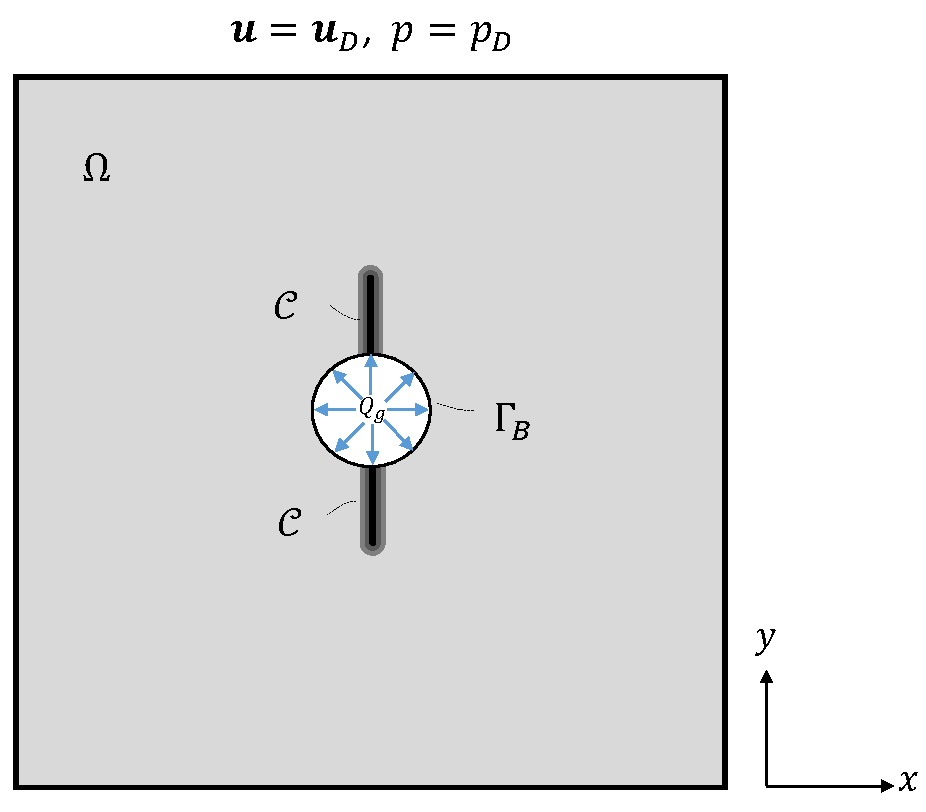
\includegraphics[width=0.8\textwidth]{omega_insitu2}
	\caption{A bounded reservoir domain $\Omega$ with a lower-dimensional crack $\mathcal{C}\in\mathbb{R}^{\eta-1}$ (left) and its diffuse approximation.}
	\label{Fig:comput_domain}
\end{figure}
\comment{We also need to define prescribed boundary condition for $T$.}
The linearized strain tensor takes the form:
\begin{equation}\label{Eq:epsilon}
	\begin{aligned}
		\bm{\varepsilon}(\bm{u})=\frac12(\nabla\bm{u}+\nabla\bm{u}^T)
	\end{aligned}
\end{equation}
which can be decomposed into two parts:
\begin{equation}\label{Eq:epsilon_decomp}
\begin{aligned}
	\bm{\varepsilon}(\bm{u}) = \bm{\varepsilon}_e+\bm{\varepsilon}_{\theta}.
\end{aligned}
\end{equation}
Here, $\bm{\varepsilon}_e$ and $\bm{\varepsilon}_{T}$ are the elastic and thermal strain tensors, respectively. We assume that $\bm{\varepsilon}_{\theta}$ is proportional to the temperature $\theta$ via:
\begin{equation}\label{Eq:epsilon_theta}
	\begin{aligned}
		\bm{\varepsilon}_{\theta} = \beta(\theta-\theta_0)\mathbf{1},
	\end{aligned}
	\end{equation}
where $\theta_0$ is a reference temperature, $\beta$ is the linear expansion coefficient of the material, and $\mathbf{1}$ is the {second-order} identity tensor.

The energy of a poroelastic medium $\Omega$ with a crack $\mathcal{C}$ reads:
\begin{equation}\label{Eq:E}
\begin{aligned}
E(\bm{u},\mathcal{C}):= \frac12 \int_{\Omega\setminus\mathcal{C}} \mathbb{C}\left(\bm{\varepsilon}_e(\bm{u})-\frac{\alpha}{3K}p\mathbf{1}\right):\left(\bm{\varepsilon}_e(\bm{u})-\frac{\alpha}{3K}p\mathbf{1}\right)\; d\Omega - W(\bm{u}),
\end{aligned}
\end{equation}
where $\mathbb{C}\in\mathbb{R}^4$ denotes the fourth-order Gassman tensor, and $\alpha\in[0,1]$ and $p$ are the Biot's coefficient and the pore pressure, respectively. Also, $K=E/[3(1-2\nu)]$ where $E$, $\nu$ are Young's modulus and Poisson's ratio, respectively.
The external work $W(\bm{u})$ is defined as:
\begin{equation}\label{Eq:External}
	\begin{aligned}
		W(\bm{u}):=\int_{\Omega} \bm{b} \cdot \bm{u} \; d\Omega+\int_{\Gamma_N} \bm{t}_N\cdot \bm{u} \; d\Gamma - \int_{\mathcal{C}} p\bm{n}\cdot[\bm{u}] \; d\Gamma,
	\end{aligned}
\end{equation}
where $\bm{n}\cdot[\bm{u}]\geq 0$ represents the displacement discontinuity on the fracture surface so that the term $\int_{\mathcal{C}} p\bm{n}\cdot[\bm{u}] \; d\Gamma$
%third term on the right hand side of \eqref{Eq:External}
is the work done by the absorbed fluid on the fracture surface.

The variational approach to fracture first proposed by Francfort and Marigo \cite{bourdin2008variational} defines the total energy as the sum of the potential energy and the surface energy required to create a fracture set $\mathcal{C}$. Let $\mathcal{H}^{\eta-1}(\mathcal{C})$ denote the lower-dimensional Hausdorff measure of $\mathcal{C}$. Taking the constant $G_c\in\mathbb{R}^+$ as the strain energy released per unit length of fracture extension, the total energy will be formed as:
\begin{equation}\label{Eq:Pi}
	\begin{aligned}
		\Pi[\bm{u},\mathcal{C}]=E(\bm{u},\mathcal{C})+G_c\mathcal{H}^{\eta-1}(\mathcal{C}).
	\end{aligned}
\end{equation}
In the variational setting, the Griffith criteria will be the
minimum of the total energy \eqref{Eq:Pi} with respect to any admissible displacement field $\bm{u}$ and any fracture set $\mathcal{C}$ subject to an irreversibility condition, i.e., the crack can never heal.

\subsubsection{Regularized variational formulation of brittle fracture}
To develop a numerical method to approximate \eqref{Eq:Pi}, we need to replace the sharp description of crack $\mathcal{C}$ with a phase field representative, where the phase field is denoted as $d:\Omega\rightarrow[0,1]$. Following the approach presented by Ambrosio and Tortorelli \cite{ambrosio1990approximation, ambrosio1992approximation}, one can approximate $\mathcal{H}^{\eta-1}(\mathcal{C})$ with the help of an elliptic functional as:
\begin{equation}\label{Eq:Gamma_ell}
\begin{aligned}
\mathcal{C}_\ell[d]:=\frac{1}{4c_{\omega}}\int_\Omega\left(\frac{\omega(d)}{\ell} + \ell \nabla d\cdot\nabla d\right) d\Omega,  
\end{aligned}
\end{equation}
%where $d:\Omega\rightarrow[0,1]$ is the phase field parameter. 
In particular, regions with $d = 0$ and $d = 1$ correspond to the intact and fully broken materials, respectively.
We denote by $\ell>0$ the regularization length scale, which may also be interpreted as a material property, e.g., the size of the process zone.
In \eqref{Eq:Gamma_ell}, we consider $c_\omega=\int_{0}^{1} \sqrt{\omega(d)}$ as a normalization constant such that as $\ell\rightarrow 0$, $\mathcal{C}_\ell[d]$ converges to the length of sharp crack $\mathcal{H}^{\eta-1}(\mathcal{C})$. Also, we choose $\omega(d)=d^2$, see \cite{tanne2018crack, Bourdin2014014301} for more elaborations.

The solid endures partial loss of stiffness due to the presence of fractures. To model this effect, the poroelastic energy needs to be degraded with respect to the evolution of the phase field. Also note that as the damaged material responds differently to tension and compression, we should let only a part of the poroelastic energy be degraded. Following \cite{amor2009regularized}, we assume that both volumetric expansion and deviatoric deformation contribute to crack propagation but not volumetric compression. 
A decomposition of $\bm{\varepsilon}_e$ into volumetric and deviatoric components reads:
\begin{equation}
	\begin{aligned}
		\vol\bm{\varepsilon}_e := \frac{1}{3} (\trace\bm{\varepsilon}_e) \mathbf{1}, \quad
		\dev\bm{\varepsilon}_e := \bm{\varepsilon}_e - \vol\bm{\varepsilon}_e,
	\end{aligned}
\end{equation}
where $\vol\bm{\varepsilon}_e$ will also be decomposed into expansion and compression parts such that
\begin{equation}
	\begin{aligned}
		\vol\bm{\varepsilon}_e=\vol_+\bm{\varepsilon}_e+\vol_-\bm{\varepsilon}_e, \quad \vol_{\pm}\bm{\varepsilon}_e=\frac{1}{\eta}\langle \trace \bm{\varepsilon}_e \rangle_{\pm}\mathbf{1},
	\end{aligned}
\end{equation}
where $\langle a\rangle_\pm:=\left(|a|\pm a\right)/2$ for all $a\in\mathbb{R}$.
%On this basis, we can rewrite \eqref{Eq:E} as:
On this basis, we rewrite \eqref{Eq:E} with decomposition of the poroelastic energy into expansion/compression volumetric and deviatoric parts as:
\begin{equation*}\label{Eq:E_Amor}
	\begin{aligned}
		E(\bm{u},\mathcal{C})&:= \frac12 \int_{\Omega\setminus\mathcal{C}} \mathbb{C}\Big\langle\vol\bm{\varepsilon}_e-\frac{\alpha}{3K}p\mathbf{1}\Big\rangle_{+}:\Big\langle\vol\bm{\varepsilon}_e-\frac{\alpha}{3K}p\mathbf{1}\Big\rangle_{+}\; d\Omega \\&+
		\frac12 \int_{\Omega\setminus\mathcal{C}} \mathbb{C}\Big\langle\vol\bm{\varepsilon}_e-\frac{\alpha}{3K}p\mathbf{1}\Big\rangle_{-}:\Big\langle\vol\bm{\varepsilon}_e-\frac{\alpha}{3K}p\mathbf{1}\Big\rangle_{-}\; d\Omega \\&+ \int_{\Omega\setminus\mathcal{C}} \mathbb{C}\dev\bm{\varepsilon}_e:\dev\bm{\varepsilon}_e\; d\Omega - W(\bm{u}),
	\end{aligned}
\end{equation*}
To take into account any pre-existing crack, we define $\Gamma_d\subset\overline{\Omega}$ to be a set with Hausdorff dimension $\eta-1$, and $d_0:\Gamma_d\rightarrow[0,1]$ as the Dirichlet boundary condition for $d$. Thus, we define the affine space of the admissible $\bm{u}$ and $d$ fields:
\begin{equation}\label{Eq:Dissipative_admissible}
\begin{aligned}
\mathscr{S}_u &:= \left\{\bm{u}\in H^1\left(\Omega; \mathbb{R}^\eta\right) \middle|
\bm{u} = \bm{u}_D \text{ on } \Gamma_D
\right\}, \\
\mathscr{S}_d &:= \left\{d\in H^1(\Omega) \middle|
0 \le d \le 1 \text{ a.e.}, d = d_0 \text{ on } \Gamma_d
\right\}. \\
%\mathscr{S}_d &:= H^1(\Omega).
\end{aligned}
\end{equation}
On this basis, the regularized variational formulation for brittle fracture of the solid reads: Find $\left(\bm{u}\times d \right)\in\mathscr{S}_{\bm{u}}\times\mathscr{S}_d$ that minimizes the following total energy:
\begin{equation}\label{Eq:Dissipative_functional}
\begin{aligned}
\Pi_{\ell}(\bm{u},d)&:= \frac12 \int_{\Omega} \mathbb{C}\Big\langle(1-d)\vol\bm{\varepsilon}_e-\frac{\alpha}{3K}p\mathbf{1}\Big\rangle_{+}:\Big\langle(1-d)\vol\bm{\varepsilon}_e-\frac{\alpha}{3K}p\mathbf{1}\Big\rangle_{+}\; d\Omega \\&+
\frac12\int_{\Omega}\mathbb{C}\Big\langle\vol\bm{\varepsilon}_e-\frac{\alpha}{3K}p\mathbf{1}\Big\rangle_{-}:\Big\langle\vol\bm{\varepsilon}_e-\frac{\alpha}{3K}p\mathbf{1}\Big\rangle_{-}\; d\Omega \\&+
\int_{\Omega} g(d)\mathbb{C}\dev\bm{\varepsilon}_e:\dev\bm{\varepsilon}_e\; d\Omega\\&+
\frac{G_c}{4c_{\omega}}\int_\Omega \left(\frac{\omega(d)}{\ell} + \ell \nabla d\cdot\nabla d\right)\;d\Omega- W(\bm{u}),
\end{aligned}
\end{equation}
\comment{I should add appropriate description for $(1-d)$.}
where $g(d)$ is a degradation function that satisfies $g(0)=1$, $g(1)=0$, and $g'(d)<0$. A usual choice is $g(d)=(1-d)^2$ \cite{Bourdin2000797}. Note that the requirement $g'(d)<0$ comes from the underlying irreversibility condition (the fracture can never heal) in time:
\begin{equation}\label{Eq:irreversibility}
\partial_t d\geq 0.
\end{equation}
Consequently, modeling of fracture evolution problems leads to {inequality constraints, and sometimes gives rise to a variational inequality formulation}.
Also, note that in this regularized form, the external work in \eqref{Eq:External} is rewritten as:
\begin{equation*}
\begin{aligned}
W(\bm{u}):=\int_{\Omega} \bm{b} \cdot \bm{u} \; d\Omega+\int_{\Gamma_N} \bm{t}_N\cdot \bm{u} \; d\Gamma - \int_{\Omega} p\bm{u}\cdot\nabla d \; d\Omega,
\end{aligned}
\end{equation*}
where $\int_{\Omega} \bm{u}\cdot\nabla d \; d\Omega$ represents the fracture volume \cite{BourdinCFRAC13}.

It can be shown that when $\ell\rightarrow 0$, the regularized formulation $\Gamma-$converges to that with explicit crack representation, i.e., when $\ell\rightarrow0$, the solution to the minimization problem \eqref{Eq:Dissipative_functional} $\Gamma$-converges to that of $d\Pi[\bm{u},\mathcal{C}]=0$, and also $\mathcal{C}_\ell[d]$ converges to $\mathcal{H}^{\eta-1}(\mathcal{C})$. See Bourdin \emph{et al.} \cite{bourdin2008variational} for the proof of the static anti-plane case.

%\paragraph{The choice of $\ell$}
%{Based on an analytical solution for the critical tensile strength $\sigma_\text{cr}$ that a one-dimensional bar can sustain \cite{Bourdin2014014301}, we use the following equation for the choice of $\ell$:}
%\begin{equation}\label{Eq:choice_ell}
%    \begin{aligned}
%        \ell=\frac{3EG_c}{8\sigma_\text{cr}^2},
%    \end{aligned}
%\end{equation}
%where $E$ and $g_c$ can be obtained from regular experiments, while $\sigma_\text{cr}$ can be approximated by the tensile strength $\sigma_t$. Assuming all {other} parameters are known, the formula \eqref{Eq:choice_ell} is able to estimate $\ell$, though the accuracy is unknown for more complex cases.

\subsection{Carbon dioxide as a compressible fluid} \label{Sec:CO2}
Assume the porous medium is saturated by a single-phase fluid. We denote by $\phi$ the porosity of the porous medium (the fraction of volume occupied by the fluid), and by $\rho_f,~\rho_s$ the fluid and solid density, respectively. Note that in this paper, the subscripts $s$  and $f$ refer to solid and fluid phases, respectively. The mass balance for the fluid reads:
\begin{equation}\label{Eq:Mass_fluid}
    \begin{aligned}
        \partial_t\left(\phi\rho_f\right)  +\nabla\cdot\left(\phi\rho_f \mathbf{v}_f\right)&=0  \quad  &\text{in~} \Omega,
    \end{aligned}
\end{equation}
%\begin{equation}\label{Eq:Mass_fluid}
%\begin{aligned}
%\nabla\cdot(\phi\mathbf{v}_f)&=0 \quad &\text{in~} \Omega,
%\end{aligned}
%\end{equation}
and for the solid phase:
\begin{equation}\label{Eq:Mass_solid}
\begin{aligned}
\partial_t\left(\left(1- \phi\right) \rho_s\right) + \nabla\cdot\left(\left(1- \phi\right)\rho_s \mathbf{v}_s\right)&=0  \quad  &\text{in~} \Omega.
\end{aligned}
\end{equation}
In \eqref{Eq:Mass_fluid} and \eqref{Eq:Mass_solid}, $\mathbf{v}_f$ and $\mathbf{v}_s$ are respectively the absolute value of fluid and solid velocity in the bulk.
Multiplying \deleted{\eqref{Eq:Mass_fluid} by $\frac{1}{\rho_f}$ and }\eqref{Eq:Mass_solid} by $\frac{1}{\rho_s}$, we sum up \eqref{Eq:Mass_fluid} and \eqref{Eq:Mass_solid} to obtain:
\begin{equation*}\label{Eq:Mass_sum}
	\begin{aligned}
	&\frac{\phi}{\rho_f}\partial_t\rho_f+\frac{1}{\rho_f}\nabla\cdot\left(\phi\rho_f \mathbf{v}_f\right)+\frac{1-\phi}{\rho_s}\partial_t\rho_s\\
	&+\frac{1}{\rho_s}\left[(1-\phi)\rho_s \nabla \cdot \mathbf{v}_s+\mathbf{v}_s \cdot \nabla \left((1-\phi)\rho_s)\right)\right]=0.
	\end{aligned}
\end{equation*}
%\begin{equation*}\label{Eq:Mass_sum}
%\begin{aligned}
%\frac{1}{\rho_f}\nabla\cdot\left(\phi\rho_f \mathbf{v}_f\right)+\frac{1-\phi}{\rho_s}\partial_t\rho_s
%+\frac{1}{\rho_s}\left[(1-\phi)\rho_s \nabla \cdot \mathbf{v}_s+\mathbf{v}_s \cdot \nabla \left((1-\phi)\rho_s)\right)\right]=0.
%\end{aligned}
%\end{equation*}
By neglecting $\nabla\left(\left(1-\phi\right)\rho_s\right)$, it reads:%(see \cite{lewis1998finite}, section 2.6.3.2),
\begin{equation}\label{Eq:Mass_sum_intmediate}
	\begin{aligned}
        \frac{\phi}{\rho_f }\partial_t\rho_f+\frac{1}{\rho_f}\nabla\cdot\left(\phi\rho_f \mathbf{v}_f\right)+\frac{1-\phi}{\rho_s}\partial_t\rho_s+(1-\phi)\nabla\cdot \mathbf{v}_s=0.
	\end{aligned}
\end{equation}
%\begin{equation}\label{Eq:Mass_sum_intmediate}
%\begin{aligned}
%\frac{1}{\rho_f}\nabla\cdot\left(\phi\rho_f \mathbf{v}_f\right)+\frac{1-\phi}{\rho_s}\partial_t\rho_s+(1-\phi)\nabla\cdot \mathbf{v}_s=0.
%\end{aligned}
%\end{equation}
We introduce an intermediate term $\nabla\cdot\left(\phi\rho_f\mathbf{v}_s\right)$ as follows:
\begin{equation*}
	\begin{aligned}
    	\frac{1}{\rho_f}\nabla\cdot\left(\phi\rho_f \mathbf{v}_s\right)=\frac{1}{\rho_f}\left[\phi\rho_f\nabla\cdot\mathbf{v}_s+\mathbf{v}_s \cdot \nabla\left(\phi\rho_f\right)\right] \approx \phi\nabla\cdot\mathbf{v}_s,
    \end{aligned}
\end{equation*}
Having this, we define $\nabla\cdot\left(\phi\rho_f\mathbf{v}_f\right)$ \added{in \eqref{Eq:Mass_sum_intmediate}} as:
\begin{equation} \label{Eq:div_vrho_f}
	\begin{aligned}
	    \frac{1}{\rho_f}\nabla\cdot\left(\phi\rho_f\mathbf{v}_f\right)
    	&=\frac{1}{\rho_f}\nabla\cdot\left(\phi\rho_f \mathbf{v}_f\right)-\frac{1}{\rho_f}\nabla\cdot\left(\phi\rho_f \mathbf{v}_s\right)+\phi\nabla\cdot\mathbf{v}_s\\
	    &=\frac{1}{\rho_f}\nabla\cdot\left[\phi\rho_f\left(\mathbf{v}_f-\mathbf{v}_s\right)\right]+\phi\nabla\cdot\mathbf{v}_s.
    \end{aligned}
\end{equation}
By substituting \eqref{Eq:div_vrho_f} in \eqref{Eq:Mass_sum_intmediate}, we obtain:
\begin{equation}\label{Eq:Mass_Conserv_sum_darcy}
\begin{aligned}
\frac{\phi}{\rho_f}\partial_t\rho_f +\frac{1-\phi}{\rho_s}\partial_t\rho_s+\nabla\cdot\mathbf{v}_s+\frac{1}{\rho_f} \nabla\cdot \left[\phi \rho_f \left(\mathbf{v}_f-\mathbf{v}_s \right)\right] =0,  \quad  &\text{in~} \Omega.
\end{aligned}
\end{equation}
%\begin{equation}\label{Eq:Mass_Conserv_sum_darcy}
%\begin{aligned}
%\frac{1-\phi}{\rho_s}\partial_t\rho_s+\nabla\cdot\mathbf{v}_s+\frac{1}{\rho_f} \nabla\cdot \left[\phi \rho_f \left(\mathbf{v}_f-\mathbf{v}_s \right)\right] =0,  \quad  &\text{in~} \Omega.
%\end{aligned}
%\end{equation}
%We will rewrite each term of \eqref{Eq:Mass_Conserv_sum_darcy} in terms of $\bm{u}, p, T$.

The first term on the left hand side of \eqref{Eq:Mass_Conserv_sum_darcy} can be written as:
\begin{equation}\label{Eq:diff_rho_f}
\begin{aligned}
\frac{\phi}{\rho_f}\partial_t\rho_f = \frac{\phi}{\rho_f} \left[ \frac{\partial \rho_f}{\partial p}\partial_t p+\frac{\partial \rho_f}{\partial T}\partial_tT\right] = \phi \left[ \beta_p \partial_t p+ \beta_T \partial_tT\right],
\end{aligned}
\end{equation}
where $\beta_p=\rho_f{\partial\rho_f}/{\partial p}$, and $\beta_T=\rho_f{\partial\rho_f}/{\partial T}$.
\comment{Here, I should add more explanations for water.}
%Under non-isothermal conditions, the gas density varies significantly with both pressure and temperature. We {capture} this by an equation of state (EOS) \cite{mahmoud2014development}:
%\begin{equation} \label{Eq:EOS}
%\rho_g\left( p,T\right)  =\frac{Mp}{Z\left( p,T\right) RT},
%\end{equation}
%where $M$ denotes the gas molecular weight, and $R$ is the general gas constant. Also, $Z$ is obtained from the following:
%\begin{equation*} \label{Eq:Z_EOS}
%Z=\left(0.702e^{-2.5T_{pr}} \right) p_{pr}^2 -\left(5.52e^{-2.5T_{pr}} \right) p_{pr}+\left(0.044 T_{pr}^2 -0.164T_{pr} +1.15\right).
%\end{equation*}
%Here, $p_{pr}=p/p_c$ and $T_{pr}=T/T_c$ are the reduced pressure and temperature, respectively. Note also $p_c$ and $T_c$ denote the critical pressure and temperature.
%On this basis, we rewrite $\beta_p$ and $\beta_T$ as follows:
%\begin{equation} \label{Eq:partial_density_p_T}
%\begin{aligned}
%\beta_p=\frac{1}{\rho_g}\frac{\partial \rho_g}{\partial p} &= \frac{1}{p}- \frac{1}{Z} \frac{\partial Z}{\partial p}, \\
%\beta_T= \frac{1}{\rho_g}\frac{\partial \rho_g}{\partial T} &= -\frac{1}{T}- \frac{1}{Z} \frac{\partial Z}{\partial T}.
%\end{aligned}
%\end{equation}
%\comment{Here, we need an equation of state for water ($\rho=\rho(p,T)$).}
The {second} term on the left hand side of \eqref{Eq:Mass_Conserv_sum_darcy} reads \cite{lewis1998finite}: %see \cite{lewis1998finite}, Equation 2.190)
\begin{equation}\label{Eq:diff_rho_s}
\begin{aligned}
\frac{1-\phi}{\rho_s} \partial_t\rho_s= \left(\alpha-\phi \right) \frac{1}{K_s} \partial_t p -\beta_s\left(\alpha-\phi \right) \partial_t T - \left(1-\alpha \right)  \nabla \cdot \mathbf{v}_s,
\end{aligned}
\end{equation}
%\comment{Is $K_s$ the same as $k$ in \eqref{Eq:E}?}
where {$K_s$ denotes the bulk modulus of the grain material}, $\beta_s=\frac{1}{\rho_s}\frac{\partial\rho_s}{\partial T}$ is the thermal expansion coefficient for the solid, and $T$ is the absolute temperature.

The {third} term on the left hand side of \eqref{Eq:Mass_Conserv_sum_darcy} (also the last term of \eqref{Eq:diff_rho_s}) can be written as follows \cite{merxhani2016introduction}:
\begin{equation} \label{Eq:solid velocity}
\begin{aligned}
\nabla \cdot \mathbf{v}_s=\nabla \cdot \dot{\bm{u}}= \left(\dot{\nabla}\cdot\bm{u}\right)=\partial_t\left(\vol\bm{\varepsilon}_e\right).
\end{aligned}
\end{equation}

The {forth} term on the left hand side of \eqref{Eq:Mass_Conserv_sum_darcy} can be written in the form of Darcy's law. This law indicates a linear relationship between the relative velocity of fluid to solid and the head pressure gradient:
\begin{equation}\label{Eq:Darcy_law}
\begin{aligned}
\mathbf{q} = \phi \left(\mathbf{v}_f-\mathbf{v}_s \right) = -\frac{\kappa}{\mu} \nabla p,
\end{aligned}
\end{equation}
where $\kappa$ is the permeability of rock, and $\mu$ is the dynamic fluid viscosity. 
Note that we neglect the effect of gravity in Darcy's law. %($\rho_f g \nabla z$)

By substituting \deleted{\eqref{Eq:diff_rho_f}, }\eqref{Eq:diff_rho_s}, \eqref{Eq:solid velocity}, and \eqref{Eq:Darcy_law} in \eqref{Eq:Mass_Conserv_sum_darcy}, the governing equation for CO$_2$ flow is written as follows:
\begin{equation}\label{Eq:General_pressure}
\begin{aligned}
\left[\phi\beta_p +\frac{\alpha-\phi}{K_s}\right]\partial_t p+\left[\phi\beta_T-\beta_s(\alpha-\phi)\right]\partial_t T\\+\alpha \partial_t(\vol\varepsilon)+\frac{1}{\rho_f}\nabla\cdot \left(\rho_f\mathbf{q}\right)=0 \quad &\text{in~} \Omega,\\
\rho_f\bm{q} \cdot \mathbf{n} =- \quad  &\text{on~} \Gamma_B,\\
p = p_D \quad &\text{on~}\Gamma_P.
\end{aligned}
\end{equation}
%\begin{equation}\label{Eq:General_pressure}
%\begin{aligned}
%\frac{\alpha-\phi}{K_s}\partial_t p-\beta_s(\alpha-\phi)\partial_t T+\alpha \partial_t(\vol\varepsilon_e)+\nabla\cdot\mathbf{q}=0 \quad &\text{in~} \Omega,\\
%\bm{q}\cdot\mathbf{n} =-Q_f \quad  &\text{on~} \Gamma_B,\\
%p = p_D \quad &\text{on~}\Gamma_P,\\
%T = T_D \quad &\text{on~}\Gamma_T.
%\end{aligned}
%\end{equation}
%where $\Gamma_P=\partial\Omega\setminus\Gamma_B$.

%\subsubsection{Calculation of $k$}
\paragraph{Change of permeability} As the crack initiates, the permeability of the solid matrix increases inside the crack. To incorporate this effect into our model, 
we correlate the permeability to phase field by:
\begin{equation} \label{Eq:k_0}
\kappa(d)=\kappa_0+d\left(\kappa_c-\kappa_0 \right),
\end{equation}
where $\kappa_0$, $\kappa_c$ are the permeability of the intact material and the crack, respectively. Hence, a change of permeability will be assumed between the intact porous medium ($d=0$) and the crack ($d=1$). In \eqref{Eq:k_0}, $\kappa_c={w_c^2}/{12}$ where $w_c$ is the fracture width. 
Following \cite{heider2018modeling}, $w_c$ in a 2D setting can be estimated at each quadrature point as:
\begin{equation*}
w_c=\sqrt{\left[h_e\left(1+\varepsilon_{11}\right)n_{c1}\right]^2+\left[h_e\left(1+\varepsilon_{22}\right)n_{c2}\right]^2},
\end{equation*}
where $h_e$ denotes the mesh size, $\varepsilon_{ii}$ are the components of strain tensor $\bm{\varepsilon}$, and $\bm{n}_c=\frac{\nabla d}{|\nabla d|}=n_{ci}\bm{e}_i$ is the normal vector to the crack path.
%\comment{We can introduce alternative approaches to calculate $w_c$, but it needs to be for each quadrature point.}

%\paragraph{Change of $\kappa_0$ by pressure and temperature} The Darcy's law in a viscous flow regime is valid for conventional reservoirs. However, when the average mean free path of the gas molecules is comparable to the pore size containing it, there is a break in continuum theory. This is evaluated by Knudsen number which is defined as the ratio of mean free path of molecules $\lambda$ to a representative path $L$, e.g., mean hydraulic radius of capillaries:
%\begin{equation}
%\begin{aligned}
%\kappa_n=\frac{\lambda}{L}, \quad \lambda=\frac{\mu}{p}\sqrt{\frac{\pi R T}{2M}}, \quad L=2\sqrt{2\tau_h}\sqrt{\frac{\kappa_{\infty}}{\phi}},
%\end{aligned}
%\end{equation}
%where $\tau_h$ is the tortuosity of the shale matrix.
%From the Knudsen number we can divide the flow as: continuous flow, slip flow, transition flow, and free molecular flow or Knudsen diffusion.
%Sheng \emph{et al.} \cite{Sheng2012} proposed a formulation which incorporates all flow regimes in one single equation to evaluate the permeability $\kappa_0$. It reads:
%%The shale permeability is also pressure dependent due to its nano-scale pore structures. Hence, the Darcy's law in its simple form is valid only for the flow in conventional reservoirs, although there are more complicated flow regimes for the shale reservoir, namely slip flow, transition flow, and Knudsen diffusion.
%%\comment{More description on flow regimes is needed.}
%%Following \cite{Civan2010, Sheng2012}, in this paper we use a formulation which incorporates all flow regimes in one single equation for the calculation of $k$:
%\begin{equation}
%\begin{aligned}
%\kappa_0=\kappa_{\infty}f(\kappa_n),
%\end{aligned}
%\end{equation}
%where $\kappa_{\infty}$ denotes intrinsic permeability. It can be measured using the pressure pulse decay \cite{Sheng2012}. Also, $f(\kappa_n)$ is written as:
%\begin{equation}
%\begin{aligned}
%f(\kappa_n)=\left(1+a\kappa_n\right)\left(1+\frac{4\kappa_n}{1-b\kappa_n}\right),
%\end{aligned}
%\end{equation}
%in which $a, b$ are dimensionless rarefaction and the slip coefficients, respectively. We find $a$ via:
%\begin{equation*}
%\begin{aligned}
%\frac{a}{a_0}-1=\frac{A}{{\kappa_n}^B},
%\end{aligned}
%\end{equation*}
%where $A, B$ are fitting constants. In this paper, we take $a_0=1.358, A=0.1780, B=0.4348$ \cite{Civan2010}.

%where $\lambda$ is given by:
%\begin{equation}
%\begin{aligned}
%\lambda=\frac{\mu}{p}\sqrt{\frac{\pi R T}{2M}}.
%\end{aligned}
%\end{equation}
%Also we take $L$ as below:
%\begin{equation}
%\begin{aligned}
%L=2\sqrt{2\tau_h}\sqrt{\frac{k_{0}}{\phi}},
%\end{aligned}
%\end{equation}
%This formulation works also for non isothermal cases.

\subsection{Energy balance equation} %\cite{Nield2017,lewis1998finite, khoei2012thermo}%%
%\todo[inline]{Mostafa: For more details see: (i) Chapter 2 of \cite{Nield2017} Equations (2.1-2.6), (ii) Chapter 1, section 2.6.3.3 \cite{lewis1998finite}, and  (iii) \cite{khoei2012thermo}}
%In order to derive the thermo-hydro-mechanical formulation, the heat transfer formulation is incorporated into the governing equations of porous saturated media using the energy conserving equation (enthalpy balance) for each phase. The governing equation of heat conduction is derived for a continuous medium from the principle of conservation of heat energy over an arbitrary fixed volume. Based on this principle, the heat increase rate of the system is equal to the summation of heat conduction and heat generation rate in a fixed volume. Applying the Fourier law of heat conduction, the energy balance equation can be written as
We assume that the solid and fluid phases are in a state of thermodynamic equilibrium, i.e., the temperature of both phases are equal at each point in the dual-phase system:
\begin{equation} \label{Eq:thermo_equilibrium}
\begin{aligned}
\theta_s=\theta_f=\theta.
\end{aligned}
\end{equation}
Based on the principle of conservation of heat energy, the heat increase rate of a system equals to sum of the heat conduction and heat generation rate in an arbitrary fixed volume.
Thus, applying the Fourier law of heat conduction, the energy balance equation for each phase of the dual-system reads:
\begin{equation}\label{Eq:energy_balance}
\begin{aligned}
\left[(c\rho)_{s,f}\frac{\partial\theta}{\partial t}+c_{s,f}\rho_{s,f}\mathbf{v}_{s,f}\cdot\nabla \theta - \nabla\cdot\left[{k}_{s,f}\nabla \theta \right] \right] &=0,
\end{aligned}
\end{equation}
where denote by $c$ the heat capacity, and by ${k}$ the heat conductivity matrix. 
Multiplying \eqref{Eq:energy_balance} by its porosity for each phase, neglecting $\mathbf{v}_{s}$, and using Darcy's law for the fluid phase, the governing equation of heat transfer in the porous media can be written as:
\begin{equation} \label{Eq:bulk_heat_transfer}
\begin{aligned}
\left(c\rho\right)_{\text{eff}} \frac{\partial \theta}{\partial t} +c_f\rho_f \mathbf{q}\cdot \nabla \theta -\nabla\cdot\left({k}_{\text{eff}}\nabla \theta\right) =0 \quad  &\text{in~} \Omega,\\
{k}_{\text{eff}}\nabla \theta\cdot\mathbf{n} =-Q_T \quad &\text{on~} \Gamma_B,\\
\theta = \theta_D \quad&\text{on~}\Gamma_T.
\end{aligned}
\end{equation}
We let:
\begin{equation} \label{Eq:eff_heat_transfer}
\begin{aligned}
(c\rho)_{\text{eff}}:=\phi(c_f\rho_f)+(1-\phi)(c_s\rho_s), \qquad
{k}_{eff}:=\phi {k}_f + (1-\phi){k}_s.
\end{aligned}
\end{equation}
Note the second term of \eqref{Eq:eff_heat_transfer} implies the effect of fluid flow on the heat transfer, as a convection term.
%By neglecting the kinematic energy in global energy balance, applying the heat conduction Fourier's law, assuming local thermal equilibrium ($T_s=T_f=T$ in each REV), fully saturated reservoir, and neglecting the effect of viscous dissipation and work down by pressure, and radiative effects, the governing equation for heat transfer in reservoir and fluid read:
%\begin{subequations}
%	\begin{align}
%	\left(1-\phi\right)\left[c\rho_s\frac{\partial T_s }{\partial t}+c\rho_s \mathbf{v}_s\cdot\nabla T_s - \nabla\cdot\left[\mathbf{k}^{T}_s\nabla T_s \right] \right] &=0 \label{eq:heat_solid} \\ \label{eq:heat_fluid}
%	\phi\left[c^p\rho_f \frac{\partial T_f}{\partial t} + c^p\rho_f \mathbf{v}_f\cdot\nabla T_f -\nabla \cdot \left[ \mathbf{k}^{T}_f\nabla T_f \right]  \right]&=0
%	\end{align}
%\end{subequations}
%where, $s$ and $f$ refer to solid and fluid, respectively; $c$ denotes the specific heat of solid; $c^p$ is the specific heat at constant pressure; $\mathbf{k}^{T}$ is the the thermal conductivity;% $q'''$ is heat production in unite volume ($W/m^3$).
%
%If we neglect the solid velocity and define the fluid velocity with the Darcy's law \cite{lewis1998finite, khoei2012thermo}, we can obtain the governing equation of heat transfer in the porous medium, by summation of \ref{eq:heat_solid} and \ref{eq:heat_fluid}:
%\begin{equation} \label{eq: bulk_heat_transfer}
%\begin{aligned}
%\left(c\rho\right)_{\text{eff}} \frac{\partial T}{\partial t} +c^p\rho_f \mathbf{q}\cdot \nabla T -\nabla\cdot\left(\mathbf{k}^T_{\text{eff}}\nabla T\right) &=0, \quad  \text{in~} \Omega,\\
%\mathbf{k}^T_{\text{eff}}\nabla T\cdot\mathbf{n} &=-Q_T, \quad \text{on~} \Gamma_B,\\
%T &= T_D, \quad\text{on~}\Gamma_T,
%\end{aligned}
%\end{equation}
%where
%\begin{equation*}
%\begin{aligned}
%\left(c\rho\right)_{\text{eff}}&=(1-\phi) c \rho_s+\phi c^p \rho_f \\
%%\left( c_p\rho\right)^{\text{fluid}}&=  \sum_{\gamma} \epsilon^{\gamma} c_p^{\gamma} \rho^{\gamma}=\phi c_p^f \rho^f \\
%\mathbf{k}^T_{\text{eff}}&=(1-\phi) \mathbf{k}^T_s \rho_s+\phi\mathbf{k}^T_f \rho_f%\\
%%\left( q'''\right) ^{\text{eff}}&=(1-\phi)q'''_s+\phi  q'''_f
%\end{aligned}
%\end{equation*}

\subsection{Summary of governing equations} The governing equations for modeling the CO$_2$ fracturing are summarized as follow: for the porous medium deformation, the functional defined in \eqref{Eq:Dissipative_functional} is minimized among $(\bm{u},d)\in \mathscr{S}_u\times\mathscr{S}_d$ under the constraint \eqref{Eq:irreversibility}, while %The lower bound $d^{n-1}$ is considered to ensure the irreversibility of the fracture. 
for the compressible fluid the boundary value problem \eqref{Eq:General_pressure} is used to solve for the pressure $p$. Also, a governing equation of heat transfer is derived from \eqref{Eq:bulk_heat_transfer}.
\section{Numerical solution}\label{sec:Num_Sol}
In this section we present an algorithm that adopts standard procedures to obtain a numerical method to solve the initial boundary value problem presented in Section \ref{sec:Math_model}. %\deleted{In the sequel we will introduce the discrete formulations in {Sections\ref{sub:weak_porous} and \ref{sec:CO2-discretization}, for the porous medium and fluid flow respectively. Note that we adopt a staggered approach to solve the coupled problem.}
%\subsection{Porous medium}
%\deleted{Here, to facilitate the numerical computation with the FEM, in \ref{sub:weak_porous} we first state the weak form. Then in \ref{sub:spatial_porous} we present the spatial discretization for the porous medium.}
%\deleted{We choose $0=t_0<t_1<\ldots<t_N=\replaced{t_f}{T}$ and seek the solution at these discrete instants. We will adopt the backward Euler method for time discretization. Now we detail how we advance from time step $n-1$ to $n$. For later convenience, let $\Delta t_n := t_n - t_{n-1}$ for $n=1,\ldots,N$. \added{As we use the same time steps,} when there is no risk of confusion, the subscript $n$ will be dropped. \replaced{It implies}{Moreover,} the field $p$ will wear a superscript $n-1$ if it refers to the solution at $t_{n-1}$, but will have no superscript if it refers to the solution at the current time step, i.e., $t_n$.} % With this specific, \eqref{Eq:General_pressure} is discretized as:
%\subsection{\deleted{Numerical algorithm}}\label{sec:Num_algo}
%\todo[inline]{YS: It is more appropriate to make Section \ref{sec:Num_algo} a subsection of Section \ref{sec:Num_Sol}.\\
%Vahid: Now it is a subsection.}
%\todo[inline]{YS: There is no clear cut comparison between monolithic and staggered approaches. Why don't we just mention how we do it and avoid commenting on the monolithic approach?\\Vahid: I agree the advantage is not so clear, but shouldn't we justify why we chose the staggered algorithm then? Now I deleted the comparison part though. See below.}
In this algorithm, a staggered approach is employed to solve the underlying equations, i.e., the solution is obtained via iteration between the variables \cite{Bourdin2000797,bourdin2008variational}. This idea is based on the fact that by fixing two variables, the problem becomes convex in the remaining unknown. However, one drawback for such an approach is that it might need many iterations to achieve convergence among the three fields.

For the problem at hand, we need to solve a coupled system consisting of mass balance for the compressible fluid and a dissipative potential energy with the phase field. We provide a fully iterative approach in which at each stage we solve for one unknown while the other two variables are fixed to their values at the last iteration. Readers are referred to Algorithm \ref{Alg:Co_2_fracking} for complete elaboration.

%\RestyleAlgo{algoruled} 
%\LinesNumbered
%\begin{algorithm}[htbp]
%	\caption{Algorithm for modeling the CO$_2$ by phase field.} \label{Alg:Co_2_fracking}
%	
%	\KwIn{  $\bm{u}_0$, $d_{0}$, $p_{0}$, $\rho_0$, $T_0$,  and $\varepsilon_{\text{tol}}$}
%	\KwOut{  $\bm{u}_n$, $d_n$, $p_n$, $T_n$, and $n= 1, \cdots,N $}
%	
%	%Construct $d$-field, $d_0$;\\
%	Set mechanical, flow, and thermal boundary conditions $\sigma_1$, $\sigma_3$, $Q_f$, and $Q_T$;\\
%	%Set $n=1$;\\
%	
%	\For()
%	{ {$n= 1 ~ to~ N$};  }{Set  $t=n\Delta t$ and $i=0$; \tcc{$i$ is an iteration counter}
%		
%		{\Repeat( ){$\varepsilon_d=\left\| d_n^{\left( m\right) }-d_{n}^{\left( m-1\right) } \right\|_{2}  <\varepsilon_{\text{tol}}$ }
%			{ 
%				$m=0$; \tcc{$m$ is another iteration counter}
%				
%				
%				
%				
%				{\Repeat( ){   $\left\| p_n^{\left( i\right) }-p_{n}^{\left( i-1\right) } \right\|_{2}  <\varepsilon_{\text{tol}} ~\textbf{and}~ \left\| \bm{u}_n^{\left( i\right) }-\bm{u}_{n}^{\left( i-1\right) } \right\|_{2}  <\varepsilon_{\text{tol}}$  }
%					{
%						Step - P: compute $p_n$ with \eqref{Eq:waekform_p};\\
%						Step - U: compute $\bm{u}_{n}$ with \eqref{Eq:Residual_i};\label{line:compute_u}\\
%						
%						
%						
%						Update $ \rho_n^{\left( i+1\right) } \leftarrow \rho(p_n^{\left( i\right) })$ with \eqref{Eq:Density_Pressure};\\
%						
%						$i+1 \leftarrow i$
%					}
%				}
%				
%				
%				Step - d: compute $d_n$ with \eqref{Eq:Residual_ii}; \\
%				$m+1 \leftarrow m$
%			}
%		}
%		
%		$\bm{u}_{n-1} \leftarrow \bm{u}_n$;\\ 
%		$p_{n-1} \leftarrow p_n$;\\ 
%		$\rho_{n-1} \leftarrow \rho_n$;\\ 
%		%$n+1 \leftarrow n$
%	}
%	
%\end{algorithm}

\RestyleAlgo{algoruled} 
\LinesNumbered
\begin{algorithm}[htbp]
	\caption{Algorithm for modeling the CO$_2$ by phase field.} \label{Alg:Co_2_fracking}
	
	\KwIn{  $\bm{u}_0$, $d_{0}$, $p_{0}$, $\rho_0$, $T_0$,  and $\varepsilon_{\text{tol}}$}
	\KwOut{  $\bm{u}_n$, $d_n$, $p_n$, $T_n$, and $n= 1, \cdots,N $}
	
	%Construct $d$-field, $d_0$;\\
	Set mechanical, flow, and thermal boundary conditions $\sigma_1$, $\sigma_3$, $Q_f$, and $Q_T$;\\
	%Set $n=1$;\\
	
	\For()
	{ {$n= 1 ~ to~ N$};  }{Set  $t=n\Delta t$ and $i=0$; \tcc{$i$ is an iteration counter}
		
%		{\Repeat( ){$\left\| p_n^{\left( i\right) }-p_{n}^{\left( i-1\right) } \right\|_{2}  <\varepsilon_{\text{tol}}$}
%			{ 
				$m=0$; \tcc{$m$ is another iteration counter}
				
				
				
				
				{\Repeat( ){   $\left\| \bm{u}_n^{\left( i\right) }-\bm{u}_{n}^{\left( i-1\right) } \right\|_{2}  <\varepsilon_{\text{tol}} ~\textbf{and}~ \left\| d_n^{\left( i\right) }-d_{n}^{\left( i-1\right) } \right\|_{2}  <\varepsilon_{\text{tol}}$  }
					{
						Step - U: compute $\bm{u}_{n}$ with \eqref{Eq:Residual_i};\label{line:compute_u}\\
						Step - d: compute $d_n$ with \eqref{Eq:Residual_ii}; \\
						
%						Update $ \rho_n^{\left( i+1\right) } \leftarrow \rho(p_n^{\left( i\right) })$ with \eqref{Eq:Density_Pressure};\\
						
						$i+1 \leftarrow i$
					}
				}
				
				{\Repeat( ){   $\left\| p_n^{\left( m\right) }-p_{n}^{\left( m-1\right) } \right\|_{2}  <\varepsilon_{\text{tol}} ~\textbf{and}~ \left\| T_n^{\left( m\right) }-T_{n}^{\left( m-1\right) } \right\|_{2}  <\varepsilon_{\text{tol}}$  }
				{
					Step - P: compute $p_n$ with \eqref{Eq:waekform_p};\\
				
%					Update $ \rho_n^{\left( i+1\right) } \leftarrow \rho(p_n^{\left( i\right) })$ with \eqref{Eq:Density_Pressure};\\
					
					Step - T: compute $T_n$ with \eqref{Eq:waekform_T};\\
					
					Update $ \rho_n^{\left( m+1\right) } \leftarrow \rho(p_n^{\left( m\right) })$ with \eqref{Eq:Density_Pressure};\\
					
					$m+1 \leftarrow m$
				}
			}
			%}
		%}
		
		$\bm{u}_{n-1} \leftarrow \bm{u}_n$;\\ 
		$p_{n-1} \leftarrow p_n$;\\ 
		$\rho_{n-1} \leftarrow \rho_n$;\\ 
		$T_{n-1} \leftarrow T_n$;\\ 
		%$n+1 \leftarrow n$
	}
	
\end{algorithm}
%\todo[inline]{YS: $d\in[0,1]$ is a wrong way to write it. The correct way is $0\le d\le 1$. Because $d$ is a function, not a single real number.\\
%Vahid: OK. So you have fixed it.}

%\todo[inline]{YS: How do we know we are using the active set method? Even if yes, why do we need to explain such a classical one? I tend to believe no; we should just mention the algorithm(s) within FEniCS we have chosen for the constrained minimization.\\Vahid: I removed the whole paragraph then. Where we name the TAO solver, I just mentioned that the solver itself imposes the lower bound.}
%
%\deleted{To ensure that $0\le d\le 1$ and also the inequality constraint \eqref{Eq:irreversibility} are imposed on the phase field, there are mainly three kinds of approaches: (a) the active-set method, (b) the penalty method \cite{gerasimov2015line} and (c) the augmented Lagrangian method \cite{Wheeler201469}. Now we briefly explain the active-set method, which we use: For each loading step, one needs to check the constraints after the stopping criterion for iteration is achieved. If no constraint is violated, then continue the computation for the next load step; otherwise, find those points that violate the constraints and set them to the appropriate upper or lower bounds for further iteration until all the constraints are satisfied.}
%
%%\todo[inline]{YS: As we have cited \cite{Logg2012}, there is no need to explain so much about FEniCS. Just keep the essence, which is the 3rd sentence below. Also ``takes care of'' is too colloquial for a paper.\\
%%	Vahid: Now I deleted the auxiliary explanations.\\
%%	YS: I objected the advertisement-like wordings for FEniCS. I changed them to neutral ones. Still I prefer simplifying the description by saying that all we need to input are the functional and its first and second derivatives and the constraints.}

We implement our method on FEniCS, an open-source finite element software \cite[pp.~173--225]{Logg2012}. Therein, the user merely needs to provide the variational form of the problem as well as the geometry and mesh information. Then, a big advantage of FEniCS is that the software itself completes all steps toward generating the global stiffness matrix.

%\todo[inline]{YS: Why don't we use line numbers to explain? Vahid: I included the line numbers for the code. The explanations are also modified accordingly.}

%\todo[inline]{YS: The upcoming three paragraphs are NOT coherent, although individually well written. Put more thoughts on their order and necessary link words.\\Vahid: It should look better now.}

Below we show an excerpt of the used FEniCS code. This piece of code performs some calculations for line \ref{line:compute_u} in Algorithm \ref{Alg:Co_2_fracking} wherein $\bm{u}$ is solved for while the other two unknowns are fixed. It first defines $\bm{\varepsilon}$, $\psi_0$, and $\psi(\bm{\varepsilon},d)$ in lines 1, 3, and 5, respectively. Then, the standard finite element shape functions are defined in line 8, and the admissible function space (\texttt{TrialFunction}), the test function space (\texttt{TestFunction}), and the unknown function $\bm{u}$ (\texttt{Function}) are defined in line 9. Afterwards, the elastic energy is introduced as a variational form in line 11. Finally, in lines 12 and 13, the code takes the first variation $\delta\Pi[(\bm{u},d);\Bar{\bm{u}}]$ \eqref{Eq:Residual_u} and the second variation $\delta^2\Pi[(\bm{u},d);\Bar{\bm{u}};\delta\bm{u}]$ \eqref{Eq:Tangent_u} and builds the nodal residual vector as \texttt{Residual\_u} and the tangent stiffness matrix as \texttt{Jacobian\_u}.
\begin{lstlisting}
def eps(u_):
return sym(grad(u_))
def psi_0(u_):
return  0.5 * lmbda * tr(eps(u_))**2 + mu * eps(u_)**2
def psi_(u_, d_):
return (1 - d_)**2 * psi_0(u_)

V_u = VectorFunctionSpace(mesh, "CG", 1)
u_, u, u_t = Function(V_u), TrialFunction(V_u), TestFunction(V_u)

energy_elastic = psi_(u_, d_) * dx
Residual_u = derivative(energy_elastic, u, u_t)
Jacobian_u = derivative(Residual, u_, u_t)
\end{lstlisting}



%\todo[inline]{YS: This is too lengthy, and ``pick up'' is too colloquial.\\Vahid: Replaced by a more brief paragraph.}
To solve the three unknowns, we select for $\bm{u}$ and $p$ the linear solver MUMPS which is convenient for solving large linear systems \cite{amestoy2000mumps}, and for $d$ the TAO optimization solver integrated into the PETSc library \cite{munson2014toolkit, petsc-user-ref}, which has the capability of solving inequality constrained optimization problems as the one at hand. Interested readers are referred to \cite{bilgen2018phase} for more information about the applied solvers.
%{As we solve for each unknowns separately, we can choose different solvers. Thus, for $\bm{u}$ using Newton's method, we pick up a linear solver like MUMPS which is convenient for the solution of large linear systems \cite{amestoy2000mumps}. For $d$, however, \eqref{Eq:Euler_d} is solved using the TAO optimization solver which is integrated into the PETSc library \cite{munson2014toolkit}, \cite{petsc-user-ref}. The fluid flow sub problem is also solved with standard Newton's method with MUMPS. Interested readers are referred to \cite{bilgen2018phase} for more elaborative information about the used solvers.}
%{As we solve for each unknowns separately, we can choose different solvers. Thus, for $\bm{u}$ using Newton's method, we pick up a linear solver like MUMPS which is convenient for the solution of large linear systems \cite{amestoy2000mumps}. For $d$, however, \eqref{Eq:Euler_d} is solved using the TAO optimization solver which is integrated into the PETSc library \cite{munson2014toolkit, petsc-user-ref}. The fluid flow sub problem is also solved with standard Newton's method with MUMPS. Interested readers are referred to \cite{bilgen2018phase} for more elaborative information about the used solvers.}
%\todo[inline]{Mostafa: The statement below is deleted since we update the parameters in each iteration according to the pressure in the last iteration, not last time step.}
%\deleted{To end this session, it is also worth mentioning that although the density $\rho$ and $\replaced{\mathcal{N}}{N}$ (See Eq. \eqref{Eq:General_pressure}) are functions of $p$, for sake of simplicity and fast numerical computation, in our algorithm they are only updated once at each time interval.}

%\todo[inline]{YS: What is the difference between Algorithms 1 and 2? Also for $n$, if we can use \texttt{For}, I will prefer it over \texttt{Repeat...Until}.\\Vahid: I am discussing with Mostafa to find the best algorithm.}

%\RestyleAlgo{algoruled} 
%\LinesNumbered
%\begin{algorithm}[htbp]
%	\caption{Algorithm for modeling the CO$_2$ by phase field.} \label{Alg:Co_2_fracking}
%	
%	\KwIn{  $p_{0}$, $d_{0}$, $\bm{u}_0$, and $\rho_0$}
%	\KwOut{  $p_n^{\left( k\right)}$, $d_n^{\left( k\right)}$, and $\bm{u}_n^{\left( k\right)}$, {for $n= 1, \cdots,N $}}
%	
%	%Construct $d$-field, $d_0$;\\
%	Set flow and mechanical boundary conditions ({$\sigma_1$}, {$\sigma_3$}, and {$Q_g$});\\
%	%Set $n=1$;\\
%	
%	\For()
%	{ {$n=1~\textbf{to}~ N$};  }{Set  $t=n\Delta t$, and $k=0$, {where $k$ is iteration counter};\\ 
%		Step - P: compute $p_n^{\left( k\right)}$, \eqref{Eq:weak_pressure};\\
%						$ \rho_n \leftarrow \rho(p_n), \eqref{Eq:Density_Pressure}$\\
%		{\Repeat( ){   $\varepsilon_d=\left\| d_n^{k}-d_{n}^{k-1} \right\|_{2}  <\varepsilon_{\text{tol}}$ }
%			{ 
%				
%				
%				Step - U: compute $\bm{u}_{n}^{\left( k\right)}$, \eqref{Eq:Residual} ;\\
%				Step - d: compute $d_n^{\left( k\right)}$, \eqref{Eq:Residual}; \\
%
%
%				
%				$k+1 \leftarrow k$
%			}
%		}
%		
%		$p_{n-1} \leftarrow p_n^{\left( k\right)}$;\\ 
%		$\rho_{n-1} \leftarrow \rho_n$;\\ 
%						$\bm{u}_{n-1} \leftarrow \bm{u}_n^{\left( k\right)}$;\\
%		%$n+1 \leftarrow n$
%		}
%	
%\end{algorithm}


%\input{section_4_Num_algo_co2.tex}
%\section{Numerical examples}
\label{sec:num-examples}
In this section, we present a numerical example to demonstrate the capability of the proposed model. 
%To verify the implementation, we performed several other numerical experiments in \ref{Sec:App}.
\subsection{Mandel's problem}
This example aims to study \dots
%In the sequel, we first describe how we solved Mandel's problem with our algorithm.
Consider a 2D rectangular domain of width $2a$ and height $2b$ occupied by a saturated poroelastic material. Constant compression forces are applied on rigid impermeable plates $y=\pm b$ with a magnitude of $2F$, see the configuration in Figure \ref{Fig:mandel}. The load is applied instantaneously at $t=0^+$. At the right edge ($x = \pm a$) the sample can be drained while the lateral boundaries are free of stress.

We only model a quarter of the sample due to symmetry. The sample is assumed to be under plane strain conditions. The following boundary conditions are imposed:
\begin{eqnarray*}
	p=0 \quad &\text{on}  \quad x=a, \\
	u_2=U_2(b,t) \quad &\text{on}\quad y=b,\\
	u_1=0 \quad &\text{on} \quad x=0,\\
	u_2=0 \quad &\text{on} \quad y=0.
\end{eqnarray*}
where $U_2(b,t))$ is the value of Mandel's closed form solution at $y =  b$ \cite{abousleiman1996mandel}.
The remaining boundary conditions are traction free boundary conditions.

Based on the analytical solution, as the compression load $2F$ is imposed, an instantaneous pressure increase and the following deformation responses are expected:	
\begin{eqnarray*}
	p(x, y, 0^+) &=&\dfrac{FB(1+\nu_u)}{3a},\\
	u_1(a, y, 0^+) &=&\dfrac{F\nu_u}{2G},\\
	u_2(x, b, 0^+) &=&-\dfrac{Fb(1-\nu_u)}{2Ga}.
\end{eqnarray*}
\begin{figure}[htbp]
	\centering
	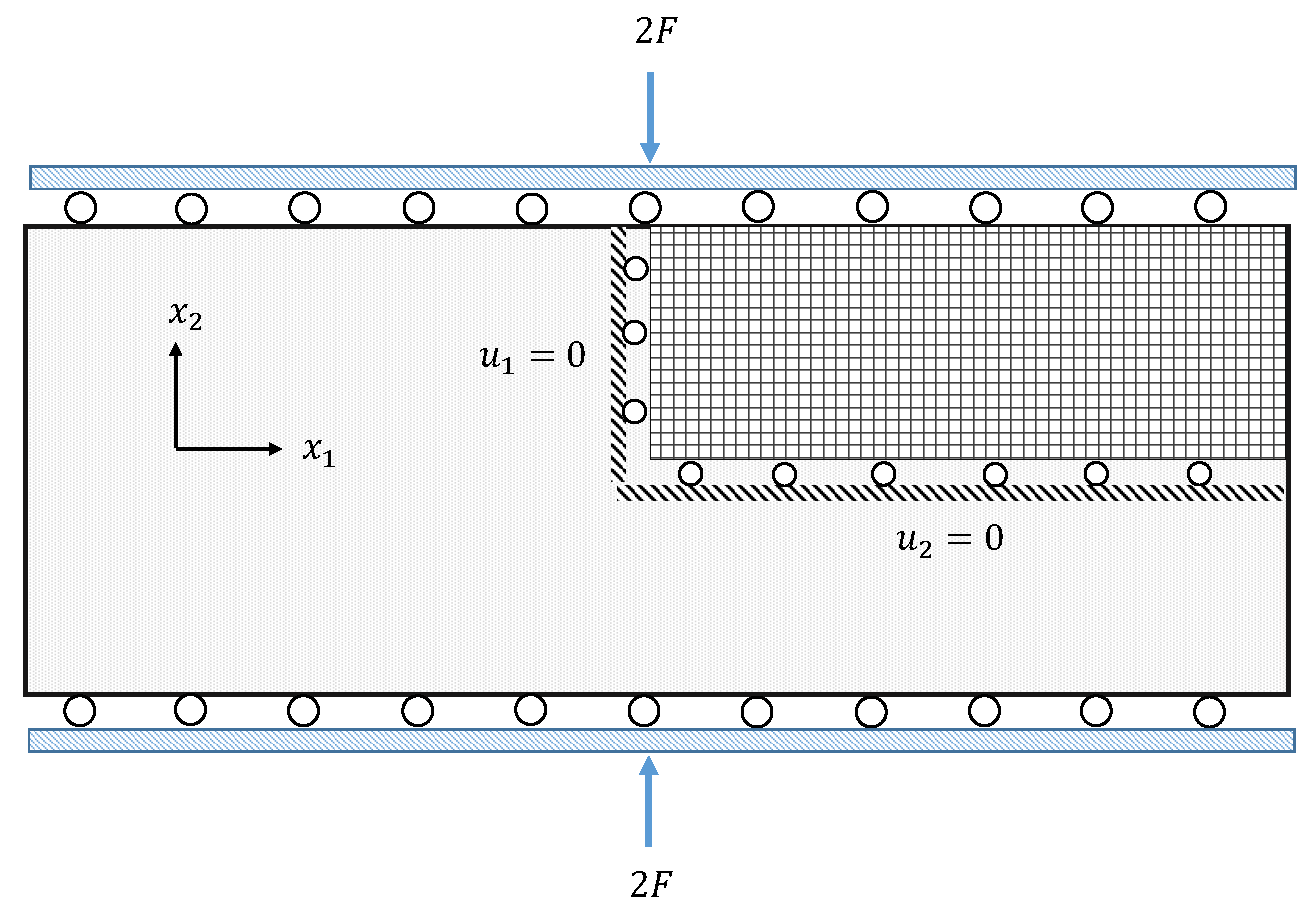
\includegraphics[width=0.8\textwidth]{MANDEL}
	\caption{Schematic view of Mandel's problem. An instantaneous compression force $2F$ is applied on the horizontal edges. Due to symmetry, only a quarter of the sample is modeled with proper boundary conditions.}
	\label{Fig:mandel}
\end{figure}
The material parameters for rock and fluid are given in Table \ref{Tab:Mandel_input}. Using our proposed algorithm in combination with the fixed-stress split method (see \cite{chukwudozie2016application, mikelic2013convergence}, which we have now also cited in the manuscript, see Section 3), we solved the numerical problem for $t_f=6$s in 600 equal time steps. Figure \ref{Fig:mandel_pressure} shows our numerical results and the analytical solution for pore pressure. Excellent agreement is observed. Figure \ref{Fig:mandel_snapshots} shows the pore pressure developed in the sample during consolidation.
\begin{table}[htbp]
	\centering
	\caption{Mandel's problem: Input parameters according to \cite{chukwudozie2016application}.}
	\begin{tabular}{l c c c}
		\hline 
		Parameters & symbol & unit& value \\
		\hline 
		Young's modulus & $E$ &MPa&  1\\
		Poisson's ratio & $\nu$ &$-$&  0.2\\
		Biot coefficient & $\alpha$ &$-$&  1.\\
		Permeability & $k_0$ &m$^2$&  1\\
		Viscosity &$\mu$ & MPa$\cdot$s &  1\\
		Length & $a$ & m &  2.5\\
		Height & $b$ & m &  1\\
		Load&$F$& MN& 2.5\\     
		Skempton coefficient &$B$& $-$& 1\\                    
		Drained Poisson's ratio&$\nu_u$& $-$&  0.5\\      
		Biot's modulus  & M & MPa & $\infty$ \\                                               
		\hline      
	\end{tabular}
	\label{Tab:Mandel_input}
\end{table}
\begin{figure}[htbp]
	\centering
	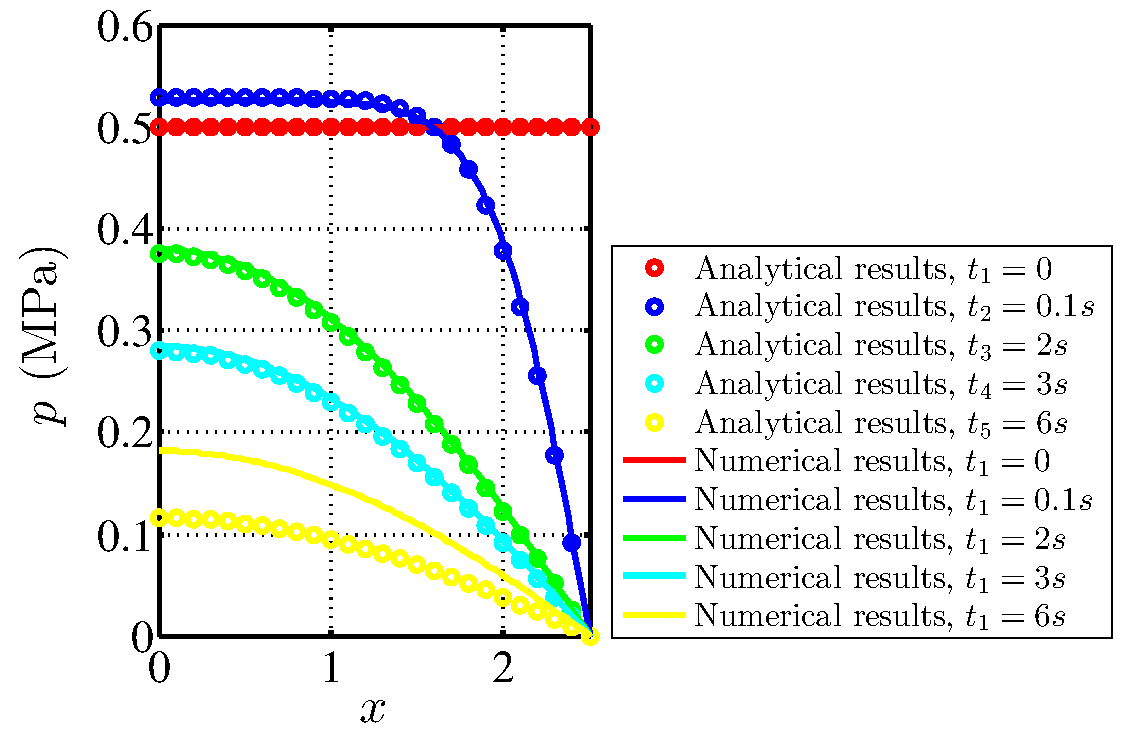
\includegraphics[width=0.8\textwidth]{mandel_pressure}
	\caption{Mandel's problem: change of pore pressure in time. Excellent agreement is observed with the analytical solution.}
	\label{Fig:mandel_pressure}
\end{figure}
\begin{figure}[htbp]
	\centering %
	\subfloat[]{
\includegraphics[width=80mm]{t9}\label{Fig:mandel_t_9}}
	\\
	\subfloat[]{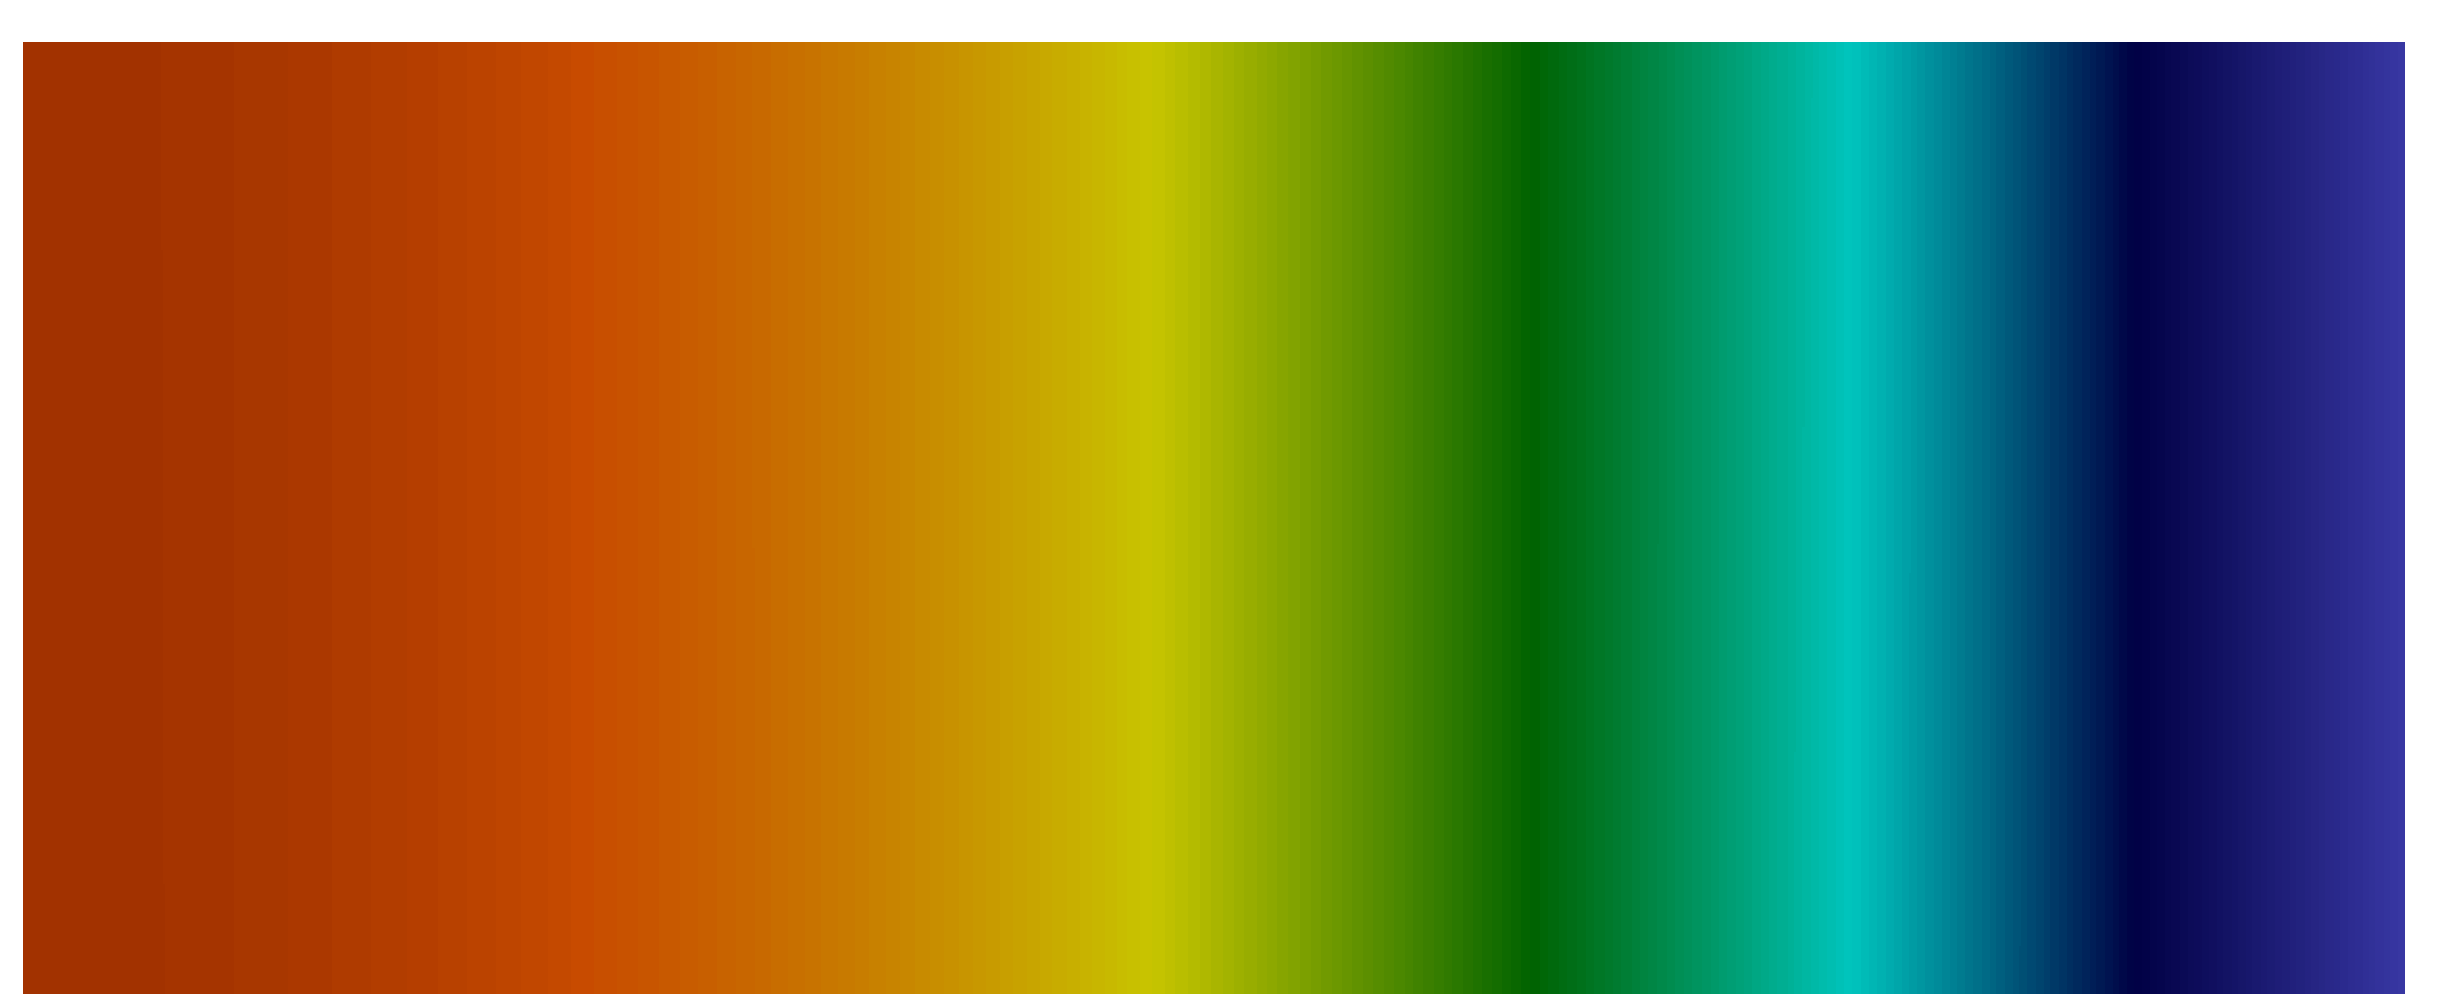
\includegraphics[width=80mm]{t199}\label{Fig:mandel_t_199}}
	\\
	\subfloat[]{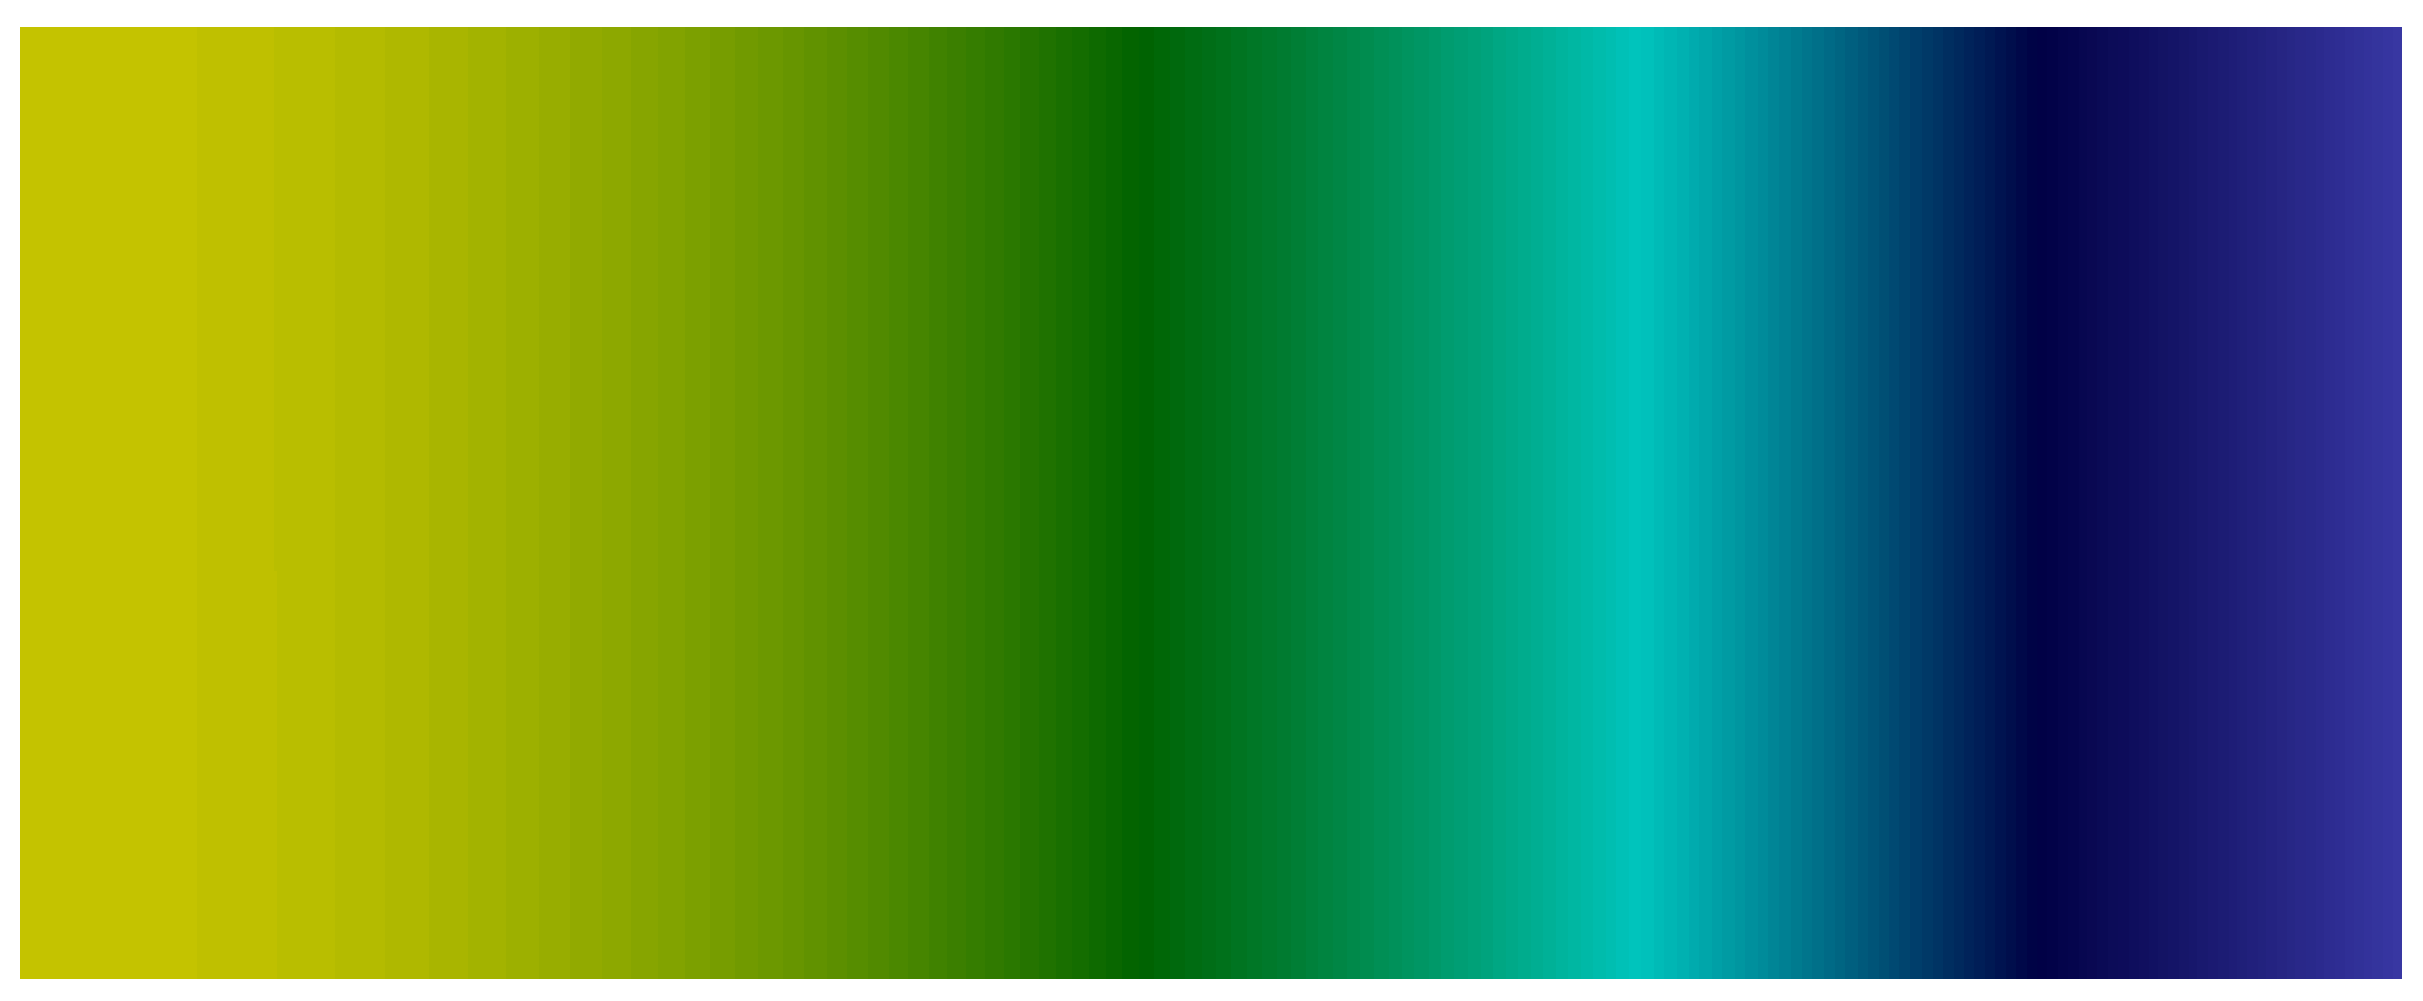
\includegraphics[width=80mm]{t299}\label{Fig:mandel_t_299}}
	\\
	\subfloat[]{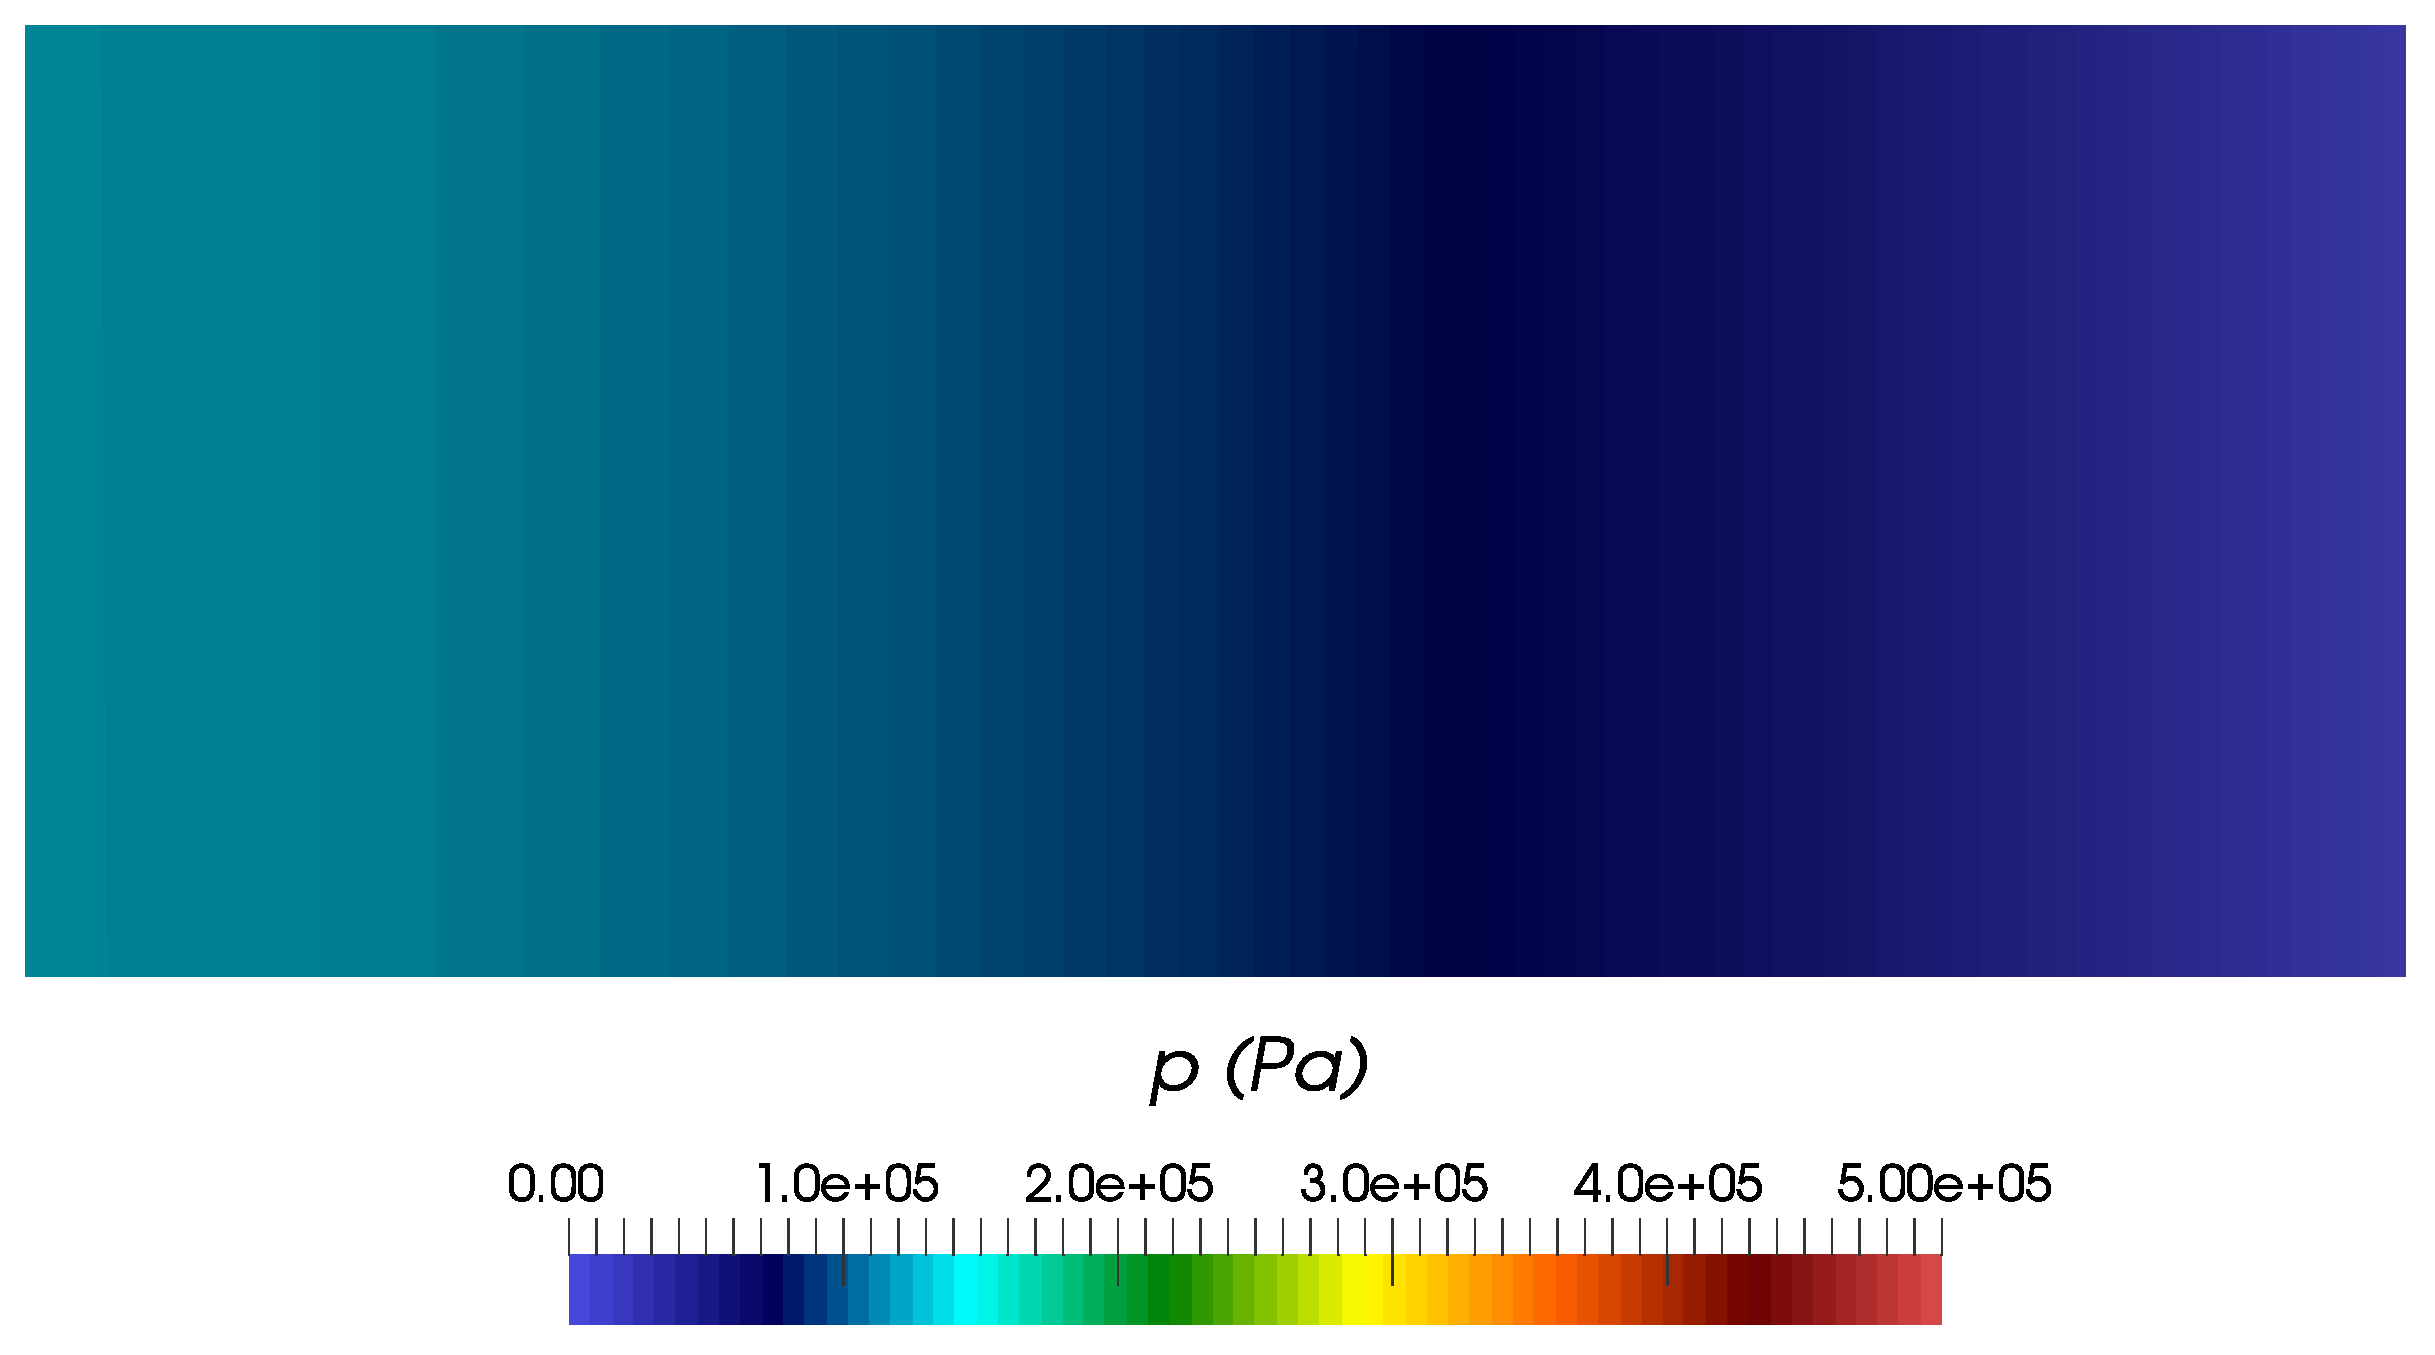
\includegraphics[width=80mm]{t599}\label{Fig:mandel_t_599}}
	\caption{Pressure profile at different stages (\ref{Fig:mandel_t_9}) $t=0.1s$, (\ref{Fig:mandel_t_199}) $t=2s$, (\ref{Fig:mandel_t_299}) $t=3s$, and (\ref{Fig:mandel_t_599}) $t=6s$). At very early stages, the pressure rises  rapidly in response to the instantaneous loading, then gradually decays to zero. %while drops until it nearly vanishes.
	}
	\label{Fig:mandel_snapshots}
\end{figure}
%A comment on Mandel's problem follows here.	
It is true that this problem is a typical poroelastic problem. However, it would somehow repeat our second verification example (see Section 4.2) where the porous flow is coupled with the porous medium's displacement. The example in Section 4.2 solved by Detourney and Cheng \cite{detournay1988poroelastic} has been used in a few works, e.g., \cite{wang2018influence, lu2013microcrack}, to verify the solution to the poroelastic response of a pressurized borehole. For these reasons, we preferred not to include Mandel's problem in the manuscript.
%\input{section_5_conclusions.tex}
%\input{section_6_Conclusions}
\clearpage
\appendix
%\renewcommand{\theequation}{A-\arabic{equation}}
%    % redefine the command that creates the equation no.
%\setcounter{equation}{0}  % reset counter  
%\input{appendix_A_verification_co2.tex}
\section{Weak forms }\label{sub:weak_form}
Here we provide weak forms useful for FEniCS implementation.

\subsection{Porous medium} \label{sub:weak_porous}
To proceed, let the test function spaces be
\begin{equation*}
    \begin{aligned}
        \mathscr{V}_u &:= \left\{\bar{\bm{u}}\in H^1\left(\Omega; \mathbb{R}^2\right) \middle|
        \bar{\bm{u}} = \mathbf{0} \text{ on } \Gamma_D
        \right\},\\
        %\mathscr{V}_d &:=\left\{\bar{d}\in H^1\left(\Omega; \mathbb{R}\right) \middle|
        %\bar{d} = {0} \text{ on } \Gamma_d
        %\right\},
        \mathscr{V}_d &:= H^1(\Omega).
    \end{aligned}
\end{equation*}
%\todo[inline]{YS: It may look better by writing \eqref{Eq:Residual} as two equations, one obtained by taking the first variation of $\bm{u}$ and the other of $d$.\\
%Mostafa: Done}
Then we derive the first variations of the energy functional \eqref{Eq:Dissipative_functional}, which will be needed for stating the weak form:
%\begin{subequations} \label{Eq:Residual}
%    \begin{align}
%	    \begin{split}
%	    \label{Eq:Residual_u}\delta \Pi_\ell & \left[(\bm{u}, d); \bar{\bm{u}} \right]
%	    := \int_\Omega \bm{\sigma}[\bm{\varepsilon}(\bm{u}), d] : \bm{\varepsilon}(\bar{\bm{u}}) \;d\Omega - \int_{\Gamma_N} \bm{t}_N\cdot \bar{\bm{u}} \; d\Gamma - \int_\Omega \bm{b} \cdot\bar{\bm{u}}\; d\Omega \\
%	    &+\int_{\Omega} \left(\alpha-1\right) \nabla \left((1-d)^2  {p}\right) \cdot \bar{\bm{u}} \; d\Omega + \int_{\Omega}  {\left(1 - d\right)}^2\nabla {p}\cdot \bar{\bm{u}}  \; d\Omega
%	    \end{split}\\
%	    \begin{split}
%	     \label{Eq:Residual_d}\delta \Pi_\ell & \left[(\bm{u}, d);  \bar{d} \right]
%	    	    := \int_{\Omega} \left(\alpha-1\right)g'(d)\bar{d} {p} \divergence{\bm{u}} \; d\Omega +	\int_{\Omega} g'(d)\bar{d}   \nabla {p} \cdot {\bm{u}} \; d\Omega 
%        \\
%	    & + \int_\Omega g'(d) \psi_+(\bm{\varepsilon}) \bar{d}  \; d\Omega +
%	    \frac{g_c}{4c_w} \int_\Omega  \left(\frac{\omega'(d)\;\bar{d}}{\ell} + 2\ell \nabla d\cdot\nabla \bar{d} \right)\;d\Omega.
%	    \end{split}
%	\end{align}
%\end{subequations}
\begin{subequations} \label{Eq:Residual}
	\begin{align}
	\begin{split}\label{Eq:Residual_i}
	\Pi_\ell &\left[(\bm{u}, d); \bar{\bm{u}} \right]:= \\&
	\int_{\Omega} \mathbb{C}\Big\langle(1-d)\vol[\bm{\varepsilon}_e(\bm{u})]-\frac{\alpha}{3K}p\mathbf{1}\Big\rangle_{+}:\Big\langle(1-d)\vol[\bm{\varepsilon}_e(\bar{\bm{u}})]-\frac{\alpha}{3K}p\mathbf{1}\Big\rangle_{+}\; d\Omega \\&+
	\int_{\Omega}\mathbb{C}\Big\langle\vol[\bm{\varepsilon}_e(\bm{u})]-\frac{\alpha}{3K}p\mathbf{1}\Big\rangle_{-}:\Big\langle\vol[\bm{\varepsilon}_e(\bar{\bm{u}})]-\frac{\alpha}{3K}p\mathbf{1}\Big\rangle_{-}\; d\Omega \\&+
	\int_{\Omega} g(d)\mathbb{C}\dev[\bm{\varepsilon}_e({\bm{u}})]:\dev[\bm{\varepsilon}_e(\bar{\bm{u}})]\; d\Omega,
%	+\frac{G_c}{4c_{w}}\int_\Omega \left(\frac{w(d)}{\ell} + \ell \nabla d\cdot\nabla d\right)\;d\Omega- W(\bar{\bm{u}}),
	\end{split}\\
	\begin{split}\label{Eq:Residual_ii}
	\delta \Pi_\ell & \left[(\bm{u}, d);  \bar{d} \right]:=\\&
	\int_{\Omega} \mathbb{C}\Big\langle(d-1)\vol[\bm{\varepsilon}_e(\bm{u})]-\frac{\alpha}{3K}p\mathbf{1}\Big\rangle_{+}:\Big\langle\bar{d}\vol[\bm{\varepsilon}_e(\bm{u})]-\frac{\alpha}{3K}p\mathbf{1}\Big\rangle_{+}\; d\Omega \\&+
	\int_{\Omega} g'(d)\bar{d}~\mathbb{C}\dev[\bm{\varepsilon}_e({\bm{u}})]:\dev[\bm{\varepsilon}_e({\bm{u}})]\; d\Omega\\&+
	\frac{G_c}{4c_{\omega}} \int_\Omega  \left(\frac{\omega'(d)\;\bar{d}}{\ell} + 2\ell \nabla d\cdot\nabla \bar{d} \right)\;d\Omega.
	\end{split}
	\end{align}
\end{subequations}
The weak form can thus be stated as: Find $\left(\bm{u}\times d \right)\in\mathscr{S}_{\bm{u}}\times\mathscr{S}_d$, such that for all admissible functions $\left(\bar{\bm{u}}\times\bar{d} \right)\in\mathscr{V}_{\bm{u}}\times\mathscr{V}_d$, $\delta\Pi_\ell\left[(\bm{u},d); \bar{\bm{u}}\right]=0$ and $\delta\Pi_\ell\left[(\bm{u},d); \bar{d}\right]=0$.

%\todo[inline]{YS: The second variation should also be written as two expressions, $ \delta^2 \Pi_\ell \left[(\bm{u}, d); \bar{\bm{u}}, \delta \bm{u}\right]$ and $\delta^2 \Pi_\ell \left[(\bm{u}, d); \bar{d}, \delta d\right]$, because we are doing a staggered algorithm.}
\todo{I should check the second variations.}
Also we take another variation from \eqref{Eq:Dissipative_functional} which will be needed for the discretized formulation:
\begin{subequations}\label{Eq:Tangent}
\begin{align}\label{Eq:Tangent_u}
\begin{split}
        \delta^2 \Pi_\ell & \left[(\bm{u}, d); \bar{\bm{u}}, \delta \bm{u}\right]
        = \int_\Omega \bm{\varepsilon}(\delta\bm{u}): \mathbb{C}[\bm{\varepsilon}(\bm{u}), d] : \bm{\varepsilon}(\bar{\bm{u}})  \;d\Omega,
        \end{split}\\
        \begin{split}
	            \delta^2 \Pi_\ell & \left[(\bm{u}, d);  \bar{d},  \delta d\right]
	    =  \int_\Omega \delta d \;g''(d) \psi_+(\bm{\varepsilon}) \bar d \; d\Omega\\ 
	    & +\int_{\Omega} \left(\alpha-1\right) g''(d)\bar{d} \; \delta d \; {p} \divergence {{\bm{u}}} \; d\Omega +\int_{\Omega}  g''(d)\bar{d} \; \delta d \; \nabla {p} \cdot {{\bm{u}}} \; d\Omega 
	    \\& +
	    \frac{G_c}{4c_w} \int_\Omega  \left[\frac{\delta d \; w''(d) \bar{d}}{\ell} + 2\ell \nabla (\delta d) \cdot \nabla \bar d \right]\;d\Omega,
	    \end{split}
\end{align}
\end{subequations}
where the fourth-order tensor $\mathbb{C}[\bm{\varepsilon}(\bm{u}), d] = \left.\frac{\partial \bm{\sigma}(\bm{\varepsilon}, d)}{\partial \bm{\varepsilon}}\right|_{\bm{\varepsilon}=\bm{\varepsilon}(\bm{u})}$ is the tangent elasticity tensor.

%\todo[inline]{YS: It looks like we don't need the following content until the beginning of Section \ref{sec:CO2-discretization}.\\
%	YS: After discussing with Mostafa on October 4, I think a better idea is, since we are using FEniCS, to keep the weak form and Jacobian in an appendix, and remove equations like \eqref{Eq:discretization} and \eqref{Eq:p_discretized}, and also remove \eqref{Eq:Residual_disc} and also the matrix formulations after it.\\Vahid: If I understood you correctly, you mean we do not need the entire subsection named ``Spatial discretization of porous medium'' \ref{sub:spatial_porous} anymore, right? I still kept the material in the tex file, and the title here though. I also changed \ref{sec:CO2-discretization} according to your comment.}
%\subsubsection{Spatial discretization of porous medium}\label{sub:spatial_porous}
%%\todo[inline]{YS: If we use a triangular mesh, then the shape functions cannot be $Q_1$.\\
%%Vahid: Yes. $Q_1$ is omitted now.}
%To discretize the problem, we divide $\Omega$ with a quasi-uniform mesh $\mathscr{T}_h$ of triangular elements for two dimensions, each member characterized by the mesh size $h$. 
%Let $\eta$ be the set of nodes of $\mathscr{T}_h$. We approximate $(\bm{u},d)$ with the standard {$P_1$} finite element basis functions associated with all nodes $i \in\eta$:
%\begin{equation}\label{Eq:discretization}
%    \begin{aligned}
%        \bm{u}(x)=\sum_{i\in\eta} \bm{N}^{\bm{u}}_{i}(x) \mathbf{u}_i,\\
%	    d(x)=\sum_{i\in\eta}N_i(x) d_i,\\
%	\end{aligned}
%\end{equation}
%where $u_i$, and $d_i$ are the displacement and phase field values at node $i$, respectively; and $\bm{N}^{\bm{u}}_{i}$ is given by
%\begin{equation*}
%    \begin{aligned}
%        \bm{N}^{\bm{u}}_{i}=\left[
%		\begin{array}{c c}
%			N_i &  0 \\
%			0 & N_i
%		\end{array}
%		\right],
%    \end{aligned}
%\end{equation*}
%where $N_i$ is the associated standard finite element shape function for each $i\in\eta$, satisfying $N_j(x_i)=\delta_{ji}$, for all $j\in\eta$, and $x_i, \mathbf{u}_i\in\mathbb{R}^{2}$ are its position vector and nodal displacement vector, respectively. The set $\eta_D \subset \eta$ is the set of nodes on  $\Gamma_D$, i.e., if $i\in\eta_D$, $\mathbf{u}_i = \mathbf{u}_D(x_i)$. The unknowns to solve are thus $\mathbf{u}_i$ for $i\in\eta\setminus\eta_D$, and $d_i$ for all $i\in\eta$. Note that we also apply the same discretization to the test functions.
%
%\paragraph{Discretized weak form} Let $\mathbf{u}\in\mathbb{R}^{2\;\#\eta}$, $d\in\mathbb{R}^{\#\eta}$ contain all entries of $\mathbf{u}_i$, ${d}_i$, respectively, for all $i\in\eta$. The discretized weak form can be written as $\mathbb{U}_i (\mathbf{u}):= \delta \Pi (\bm{u}; \bm{N}_i)=\mathbf{0}$, for all $i\in\eta\setminus\eta_D$, and $\mathbb{D}_i({d}):=\delta\Pi ({d}; {N}_i)=0$ for all $i\in\eta$. %, where $\mathbf{R}_A$. 
%Hence, the residual matrices form of \eqref{Eq:Residual} are expressed as follows:
%
%\begin{equation}\label{Eq:Residual_disc}
%	\begin{aligned}
%		\mathbb{U}_i & = \int_\Omega (\bm{B}_i)^T \bm{\sigma}[\bm{\varepsilon}(\bm{u}), d] \;d\Omega - \int_{\Gamma_N} (\bm{N}^{\bm{u}}_{i})^T\bm{t}_N \; d\Gamma - \int_\Omega (\bm{N}^{\bm{u}}_{i})^T\bm{b} \; d\Omega\\ &\quad +\int_{\Omega} (\alpha-1)\nabla\left((1-d)^2 \replaced{p}{p_B}\right) \cdot (\bm{N}^{\bm{u}}_{i}) \; d\Omega +\int_{\Omega}  (\bm{N}^{\bm{u}}_{i})^T {\left(1 - d\right)}^2\nabla \replaced{p}{p_B}  \; d\Omega\\
%	    \mathbb{D}_i &= \int_\Omega g'(d) \psi_+(\bm{\varepsilon}) N_i \; d\Omega + \frac{g_c}{4c_w} \int_\Omega  \left(\frac{w'(d) N_i}{\ell} + 2\ell \nabla d \cdot \nabla N_i \right)\;d\Omega \\& \quad+\int_{\Omega} \left(\alpha-1\right)g'(d)N_i \;\replaced{p}{p_B} \nabla \bm{u} \; d\Omega +	\int_{\Omega} g'(d) N_i \nabla \replaced{p}{p_B} \cdot \bm{u} \; d\Omega,
%	\end{aligned}
%\end{equation}
%where $\mathbb{U}_i\in\mathbb{R}^2$ and $\mathbb{D}_i \in\mathbb{R}$ represent the nodal residual vectors (also called the \emph{nodal forces} of $i$) obtained with displacement test function and phase field test function, respectively. 
%Also note that in \eqref{Eq:Residual_disc}, $\bm{\sigma}$ is understood as a 3-vector, % in 3D.
%and the strain-displacement matrices are given by:
%\begin{equation*}
%    \bm{B}_i=\left[
%	\begin{array}{c c}
% 	N_{i,x} &  0\\
% 	0 & N_{i,y} \\
% 	N_{i,y} & N_{i,x} \\
% 	\end{array}
% 	\right].
%\end{equation*}
%
%\paragraph{Tangent stiffness matrices} If a staggered algorithm is used, the tangent stiffness matrices form of \eqref{Eq:Tangent} are $\mathbf{K}_{ij}:=\partial\mathbb{U}_i/\partial\mathbf{u}_j=\delta^2\Pi[\bm{u};\bm{N}^{\bm{u}}_i, \bm{N}^{\bm{u}}_j]\in \mathbb{R}^{2\times 2}$ for all $i,j\in\eta\setminus\eta_D$ and $ \bar{\bm{K}}_{ij} :=\partial\mathbb{D}_i/\partial {d}_j=\delta^2\Pi[{d};{N}_i, {N}_j]\in \mathbb{R}$ for all $i,j\in\eta$, which can be expressed as follows:
%\begin{subequations}
%    \begin{align}
%        \bm{K}_{ij} &= \int_\Omega (\bm{B}_i)^T \bm{D} \bm{B}_j \;d\Omega,\\
%    \begin{split}
%        \bar{\bm{K}}_{ij} &= \int_\Omega \;g''(d) \psi_+(\bm{\varepsilon}) N_i N_j\; d\omega
%        + \int_{\Omega} g''(d) N_i \; N_j \; \nabla \replaced{p}{p_B} \cdot {{\bm{u}}} \; d\Omega 
%	    \\ &+ \frac{g_c}{4c_w} \int_\Omega \left[\frac{w''(d) N_i \; N_j}{\ell} + 2\ell \nabla N_i \cdot \nabla N_j \right]\;d\Omega,
%    \end{split}
%    \end{align}
%\end{subequations}
%where denote by $\mathbf{D}$ the matrix forms of the tangent elastic modulus tensor $\mathbb{C}$. Below we give $\mathbf{D}$ for different phase field models:
%\paragraph{Model A} We have $\mathbf{D}_+=\mathbf{D}_0$ and $\mathbf{D}_-=\mathbf{0}$ 
%where $\mathbf{D}_0$ for the plane strain case is defined as:
%\begin{equation*}\label{Eq:D_0}
%	    \bm{D}_{0} = \begin{bmatrix} 
%	    \lambda+2\mu & \lambda & 0 \\
%	    \lambda & \lambda+2\mu & 0 \\
%	    0 & 0 & \mu
%	   \end{bmatrix}.
%\end{equation*}
% 
%\paragraph{Model B} Let $\mathbf{1}$, be the $3\times3$ identity matrix. Then
%\[\begin{aligned}
%\mathbf{D}_+ &= KH(\trace\bm{\varepsilon}) \begin{bmatrix}
%1 & 1 & 0 \\
%1 & 1 & 0 \\
%0 & 0 & 1 
%\end{bmatrix} + 2\mu\left(\mathbf{1} - \frac13\begin{bmatrix}
%1 & 1 & 0 \\
%1 & 1 & 0 \\
%0 & 0 & 1 
%\end{bmatrix} \right),\\
%\mathbf{D}_- &= KH(-\trace\bm{\varepsilon}) \begin{bmatrix}
%1 & 1 & 0 \\
%1 & 1 & 0 \\
%0 & 0 & 1 
%\end{bmatrix} .
%\end{aligned}\]
%
%Here, $H$ is the Heaviside function such that $H(a)=1$ if $a>0$, $H(a)=0$ if $a<0$, and $H(a)=\frac12$ if $a=0$.

%\subsection{Compressible (CO$_2$) fluid flow}

\subsection{Compressible (CO$_2$) fluid flow discretization}
\label{sec:CO2-discretization}
The compressible fluid flow discretization is also done via the finite element method. We first discretize in time and then in space. We will adopt the backward Euler method for time discretization.

%\todo[inline]{YS: The same time steps or no?\\
%Vahid: Yes, the same time step. Look the changed sentence below in blue for the changes.\\
%YS: No! We cannot first introduce the discrete times and then after a few lines we say they are equally spaced. If they are equally spaced, then we say that up front! We first decide on the number of time steps, and then the discrete times and the time step are determined.\\
%Vahid: All parts are removed now.\\
%Another point: The notation $N$ is conflicted.\\
%Vahid: All parts are removed now.}
%\todo[inline]{YS: I suggest we keep $k(d)$ all along, instead of writing $k_0\exp(7d)$, to leave flexibility in the choice of the model.\\
%Vahid: OK. Now the relevant equation \eqref{Eq:weak_pressure} is modified.}
%\paragraph{Time discretization}
%\replaced{hi}{We choose $0=t_0<t_1<\ldots<t_N=\replaced{t_f}{T}$ and seek the solution at these discrete instants. We will adopt the backward Euler method for time discretization. Now we detail how we advance from time step $n-1$ to $n$. For later convenience, let $\Delta t_n := t_n - t_{n-1}$ for $n=1,\ldots,N$. \added{As we use the same time steps,} when there is no risk of confusion, the subscript $n$ will be dropped. \replaced{It implies}{Moreover,} the field $p$ will wear a superscript $n-1$ if it refers to the solution at $t_{n-1}$, but will have no superscript if it refers to the solution at the current time step, i.e., $t_n$.} With this specific, \eqref{Eq:General_pressure} is discretized as:


%\begin{equation} \label{Eq:General_pressure_time_discrete}
 %   \begin{aligned}
  %      \frac{\phi}{{N}}\frac{ p-p^{n-1}}{\Delta t}+\rho \dfrac{ \varepsilon_v-\varepsilon_v^{n-1}}{\Delta t}
%		\added{-\frac{1}{\mu}\left[\frac{k}{N}\left|\nabla p\right|^2+k\rho\Delta p+\rho\nabla k\cdot \nabla p\right]}=Q_g \; \;on \;\Omega,
%    \end{aligned}
%\end{equation}
%\Comment{YS: The equation $p \in H^1(\Omega; \mathbb{R})$ should read $p \in H^1 (\Omega)$}

%\todo[inline]{YS: Mostafa, this paragraph is taken from our previous paper. Now we are solving EQUATIONS instead of inequalities, then there is no need to say ``necessary condition.''\\Mostafa: Right. It's deleted.}
%\todo[inline]{YS: How come we have $\Gamma_B$? Is it part of $\partial \Omega$? This should have appeared in Section \ref{sec:Math_model}.\\Vahid: The related part is removed now. We have defined $\Gamma_B$ in Section \ref{sec:Math_model}.}
%\todo[inline]{YS: Why do we use $\delta p$ here but $\overline{\bm{u}}$ and $\overline{d}$? It looks like the latter is better as $\delta$ is also used in the EOS.\\Vahid: Now I changed it to $\overline{p}$.}
%\paragraph{Spatial discretization}
%Let the admissible {set} of pressure be
%\begin{equation*}
%    \begin{aligned}
%        \mathscr{S}_p &:= \left\{p \in H^1 (\Omega) \middle|
%        p = p_D\text{ on }\Gamma_D \right\}.
%    \end{aligned}
%\end{equation*}
%\todo[inline]{YS: Move $\mathscr{S}_p$ here. Again, make sure on which part of $\partial\Omega$ we are imposing $p$.\\Vahid: Done. Now we are imposing $p_D$ on $\Gamma_P$.}

To proceed, let the admissible set of pressure be:
\begin{equation*}
	\mathscr{S}_p := \left\{p \in H^1 (\Omega) \middle|
	p = p_D~\text{on}~\Gamma_P \right\}.
\end{equation*}
The test function space can be defined as:
\begin{equation*}
\mathscr{V}_{p}= \left \{{\overline{p}}\in H^1(\Omega) \middle | {\overline{p}} =0~\text{on}~\Gamma_P\right \}.
\end{equation*}
The weak form can be stated as: find $p\in\mathscr{S}_p$ such that for all admissible functions $\overline{p}\in\mathscr{V}_p$,
\begin{equation} \label{Eq:waekform_p}
    \begin{aligned}
     &\frac{1}{\Delta t} \int_{\Omega} \frac{\alpha-\phi}{K_s} \left(p-p^{n-1}\right){\overline{p}} \; d\Omega-\frac{1}{\Delta t} \int_{\Omega} \beta_s(\alpha-\phi) \left(T-T^{n-1}\right){\overline{p}} \; d\Omega\\&+\frac{\alpha}{\Delta t} \int_{\Omega} (\vol\bm{\varepsilon}_e-\left(\vol\bm{\varepsilon}_e\right)^{n-1}){\overline{p}} \; d\Omega+\int_{\Omega}  \frac{\kappa}{\mu} \nabla p \cdot \nabla {\overline{p}} \; d\Omega   
     -\int_{\Gamma_B} Q_p {\overline{p}} \; d\Gamma =0,
    \end{aligned}
\end{equation}
where $p^{n-1}$, $T^{n-1}$, and $\left(\vol\bm{\varepsilon}_e\right)^{n-1}$ are obtained from previous time step.

\subsection{Energy balance}
To proceed, let the admissible set of pressure be:
\begin{equation*}
	\mathscr{S}_T := \left\{T \in H^1 (\Omega) \middle|
	T = T_D~\text{on}~\Gamma_T \right\}.
\end{equation*}
The test function space can be defined as:
\begin{equation*}
\mathscr{V}_{T}= \left \{{\overline{T}}\in H^1(\Omega) \middle | {\overline{T}} =0~\text{on}~\Gamma_T \right \}.
\end{equation*}
The weak form can be stated as: find $T\in\mathscr{S}_T$ such that for all admissible functions $\overline{T}\in\mathscr{V}_T$:
\begin{equation} \label{Eq:waekform_T}
    \begin{aligned}
&\frac{1}{\Delta t} \int_{\Omega} \left( c\rho\right)_{\text{eff}} \left(T-T^{n-1}\right) \overline{T} \; d\Omega+\int_{\Omega} \left( c_f \rho_f \mathbf{q}\cdot \nabla T \right) \overline{T}  \; d\Omega \\&-\int_{\Omega}{k}_{\text{eff}} \nabla T \cdot \nabla \overline{T}\; d\Omega  -\int_{\Gamma_B}Q_T {\overline{T}} \; d\Gamma 
=0
    \end{aligned}
\end{equation}


\section*{Acknowledgments}
  This work is supported by the National Natural Science Foundation of China with grant \#11402146. YS also acknowledges the financial support by the Young 1000 Talent Program of China.

%\section*{References}
%% Vancouver name/year
%\bibliographystyle{model4-names}\biboptions{authoryear}
\bibliography{ref}
%\bibliography{../Revision/ref}
\end{document}